\documentclass[9pt]{beamer}

\mode<presentation> 
{ \usetheme[nat,dogma]{Frederiksberg} }

% \usepackage[danish]{babel}
\usepackage[latin1]{inputenc}
\usepackage{times}
\usepackage[T1]{fontenc}
\usepackage[english]{babel}
\usepackage{hyperref}
\usepackage{animate}
%\usepackage{multimedia}
\usepackage{francois-preamble}
\usepackage{multirow}
\usepackage{tikz}
\usetikzlibrary{shapes,arrows}
\usetikzlibrary{arrows,decorations.pathmorphing,backgrounds,fit,positioning,shapes.symbols,chains}
%\usepackage{movie15}

\newcommand{\cc}{{c\!\!,}}
\newcommand{\degr}[1]{{{#1}^\circ}}

\title{Vision and Image Processing:\\ Camera Models, Shading, Photometric Stereo}

\author[F.~Lauze] % (optional, use only with lots of authors)
{Fran{\c c}ois Lauze}

\institute[DIKU] % (optional, but mostly needed)
{
  Department of Computer Science\\
  University of Copenhagen
}

\date[2015-16 B2] % (optional, should be abbreviation of conference name)
% {Research Presentation, Diku 2006}

\definecolor{gold}{rgb}{0.95,0.83,0.0}
\definecolor{orange}{rgb}{0.95,0.7,0.0}
% \definecolor{backblue}{rgb}{0.93,0.94,0.99}
\definecolor{backblue}{rgb}{0.95,0.94,0.99}
\setbeamercolor*{background canvas}{bg=backblue} 



\newcommand{\myemph}[1]{{\color{blue}{#1}}}
\newcommand{\intrg}[1]{\int_{{#1}=-\infty}^\infty}
\newcommand{\intRR}{\int_{-\infty}^\infty}

\AtBeginSection[]
{
  \begin{frame}<beamer>{Outline}
    \tableofcontents[currentsection,currentsubsection]
  \end{frame}
}

\begin{document}
\maketitle

% would be cool with more images showing applications


%-------------------------------------------------------------------
%   Start slides
%-------------------------------------------------------------------




%----------------------------------------------



\begin{frame}
  \frametitle{Plan for today}
  \begin{itemize}
  \item Before we start, Linear Algebra Again.
  \item Motivation and a Bit of History.
  \item Camera Models, the Pinhole Camera Model.
  \item Notions of projection and projective geometry.
  \item Beyond the Pinhole Camera Model.
  \item And Before: Orthographic Projection Camera Model.
  \item A few words on Wednesday.
  \end{itemize}
\end{frame}


\section{Linear Algebra Again}
\label{sec:linalg}



\begin{frame}
  \frametitle{Matrices /linear mappings as geometric transformations}. 
  \begin{columns}
    \column{0.5\textwidth}
    \begin{center}
    Projection  on $x-y$ plane
    \end{center}
    \column{0.5\textwidth}
    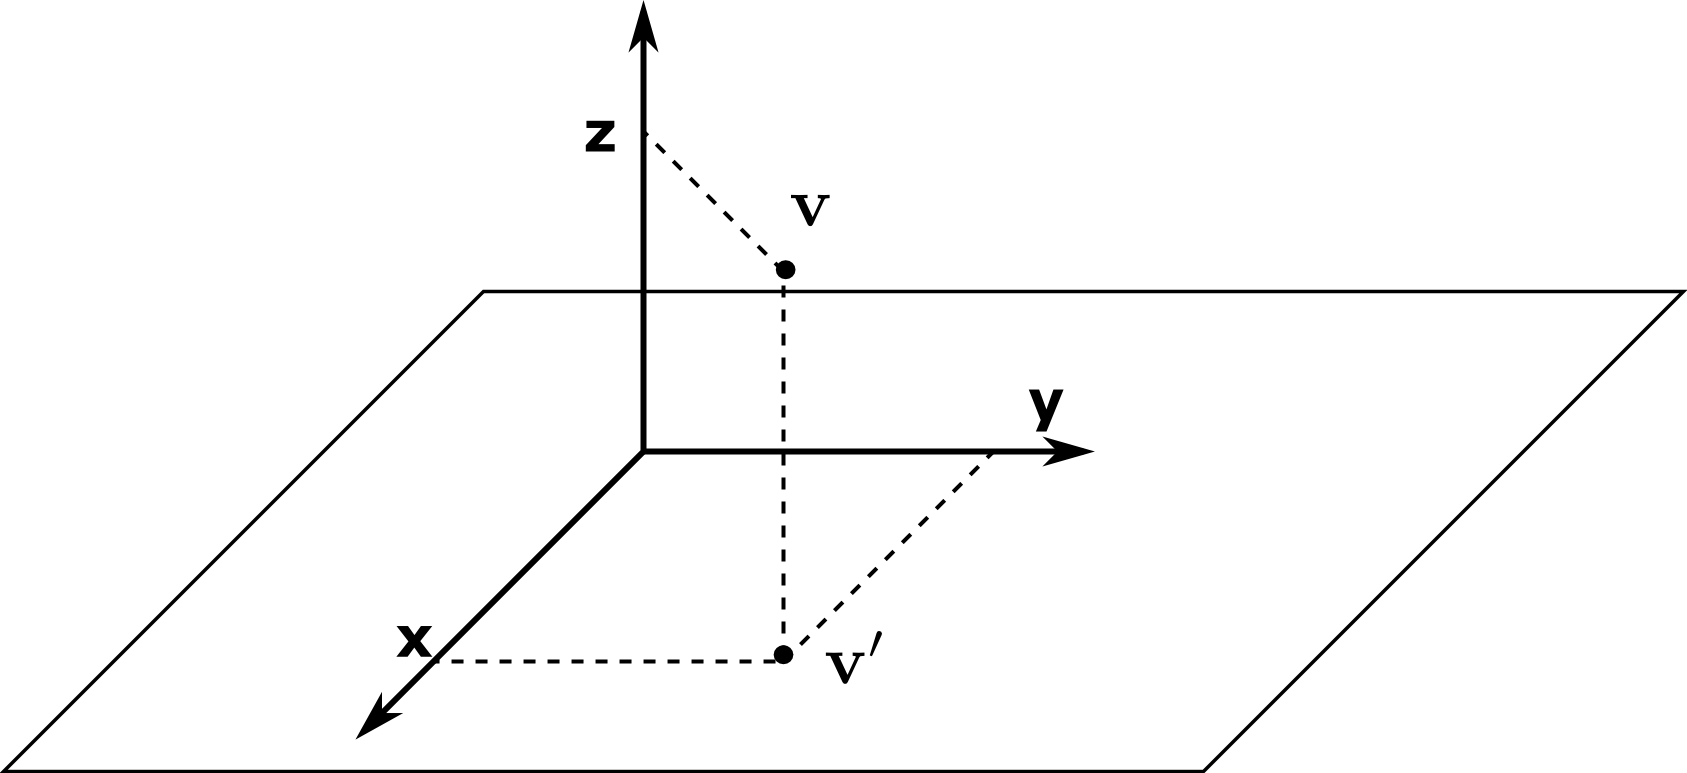
\includegraphics[width=\textwidth]{FIGURES/3dto2dproj}
  \end{columns}
  \begin{center}
    \includegraphics[width=0.9\textwidth]{FIGURES/simpletransforms}\\
    Rotation of angle $\theta$ \hfill anisotropic scaling \hfill ~~~~~~shear~~~~~~~~~~~
  \end{center}
\end{frame}

\begin{frame}
  \begin{itemize}
  \item projection $\RR^3\to\RR^2$
    $$
    F
    \begin{bmatrix}
      x \\y \\z
    \end{bmatrix}
    =
    \begin{bmatrix}
      x \\y
    \end{bmatrix},\quad F =
    \begin{bmatrix}
      1 & 0 & 0\\
      0 & 1 & 0\\
      0 & 0 & 0
    \end{bmatrix}
    $$
  \item Rotation of angle $\theta$ from $\RR^2\to\RR^2$:
    $$
    R_\theta
    \begin{bmatrix}
      x \\y
    \end{bmatrix}
    =
    \begin{bmatrix}
      x\cos\theta - y\sin\theta\\
      x\sin\theta + y\cos\theta
    \end{bmatrix},\quad
    R_\theta =
    \begin{bmatrix}
      \cos\theta & -\sin\theta\\
      \sin\theta & \cos\theta
    \end{bmatrix}
    $$
  \item Scaling by a factor $\alpha$ in $x$ and $\beta$ in $y$:
    $$
    A_{\alpha\beta}
    \begin{bmatrix}
     x\\y 
    \end{bmatrix}
    = 
    \begin{bmatrix}
      \alpha x\\
      \beta y
    \end{bmatrix},\quad
    A_{\alpha\beta} =
    \begin{bmatrix}
      \alpha & 0\\0 & \beta
    \end{bmatrix}
    $$
  \item Shear of the $y$-axis with  angle $\theta$:
    $$
    S_\theta
    \begin{bmatrix}
      x\\y
    \end{bmatrix}
    =
    \begin{bmatrix}
      x + \sin\theta y\\
      y
    \end{bmatrix},\quad
    S_\theta =
    \begin{bmatrix}
      1 &\sin\theta\\
      0 & 1
    \end{bmatrix}
    $$
  \end{itemize}
\end{frame}



% \begin{frame}
%   \frametitle{Product of Matrices}
%   \begin{itemize}
%   \item A matrix of size $m\times n$ and a matrix of size $n\times p$
%     can be multiplied to produce a matrix of size $m\times p$.
%   \item Algebraic rule: $a_{ij}$ entry $(i,j)$ of $A$, $b_{jk}$ entry $(j,k)$ of $B$
%     $$
%     A = (a_{ij})_{\substack{i=1\dots m\\j=1\dots n}},\quad 
%     B = (b_{jk})_{\substack{j=1\dots n\\k=1\dots p}}
%     $$
%     Denote entry $(i,k)$ of product $C = AB$ by $c_{ik}$:
%     $$
%     c_{ik} = \sum_{j = 1}^n a_{ij}b_{jk}
%     $$
%   \item Matrix vector multiplication is in fact a special case of it!
%   \item Example
%     $$
%     \begin{bmatrix}
%       2 & 2\\
%       1 & 3\\
%       1 & -1\\
%     \end{bmatrix}
%     \begin{bmatrix}
%       1 & 3 & 0\\
%       -2 & 0 & 1
%     \end{bmatrix}
%     = \onslide<2->
%     \begin{bmatrix}
%       -2 & 6 & 2\\
%       -5 & 3 & 3\\
%       3 & 3 & -1
%     \end{bmatrix}
%     $$
%   \item What does matrix multiplication means?
%   \end{itemize}
% \end{frame}

% \begin{frame}
%   \frametitle{Meaning of the Product}
%   \begin{itemize}
%   \item $M$ and $N$ the linear mappings $
%     \begin{bmatrix}
%       2 & 2\\
%       1 & 3\\
%       1 & -1\\
%     \end{bmatrix}
%     $ and 
%     $
%     \begin{bmatrix}
%       1 & 3 & 0\\
%       -2 & 0 & 1
%     \end{bmatrix}
%     $
%   \item
%     Apply $N$ to $
%     \bv = \begin{bmatrix}
%       x \\ y \\ z
%     \end{bmatrix}
%     $
%     and $M$ to the result:
%     $$
%     N \bv = \begin{bmatrix}
%       1 & 3 & 0\\
%       -2 & 0 & 1
%     \end{bmatrix}\begin{bmatrix}
%       x \\ y \\ z
%     \end{bmatrix}
%     = 
%     \begin{bmatrix}
%       x + 3y\\
%       -2x + z
%     \end{bmatrix}
%     $$
%     \item and{\small
%       $$
%       \begin{bmatrix}
%       2 & 2\\
%       1 & 3\\
%       1 & -1\\
%     \end{bmatrix}
%      \begin{bmatrix}
%       x + 3y\\
%       -2x + z
%     \end{bmatrix}
%     =\onslide<2->
%     \begin{bmatrix}
%       -2x+6y+2z\\
%       -5x + 3y+3z\\
%       3x + 3y-z
%     \end{bmatrix}
%     =\onslide<3->
%     \begin{bmatrix}
%       -2 & 6 & 2\\
%       -5 & 3 & 3\\
%       3 & 3 & -1
%     \end{bmatrix}
%     \begin{bmatrix}
%       x\\y\\z
%     \end{bmatrix}
%     $$}
%     % \item VIP (Very Important Property) \myemph{Matrix multiplication correspomds to chaining linear transforms}!
%   \end{itemize}
% \end{frame}


% \begin{frame}
%   \frametitle{Matrix Product as Chain Application of Linear Mappings}
%   \begin{itemize}
%   \item We found that 
%     $$
%     M\left (N\bv\right) = \udesc{\text{Matrix product}}{M N}\bv
%     $$
%   \item Very Important Property: Matrix product corresponds to chain application (composition) of linear mappings!
%   \end{itemize}\vfill
%   \begin{center}
%     \large
%     Read the Linear Algebra Tutorial and Reference on Absalon!   
%   \end{center}
%   This will also be useful for other courses!
% \end{frame}


\section{Introduction}

\begin{frame}
  \frametitle{Motivation}
  \begin{center}
    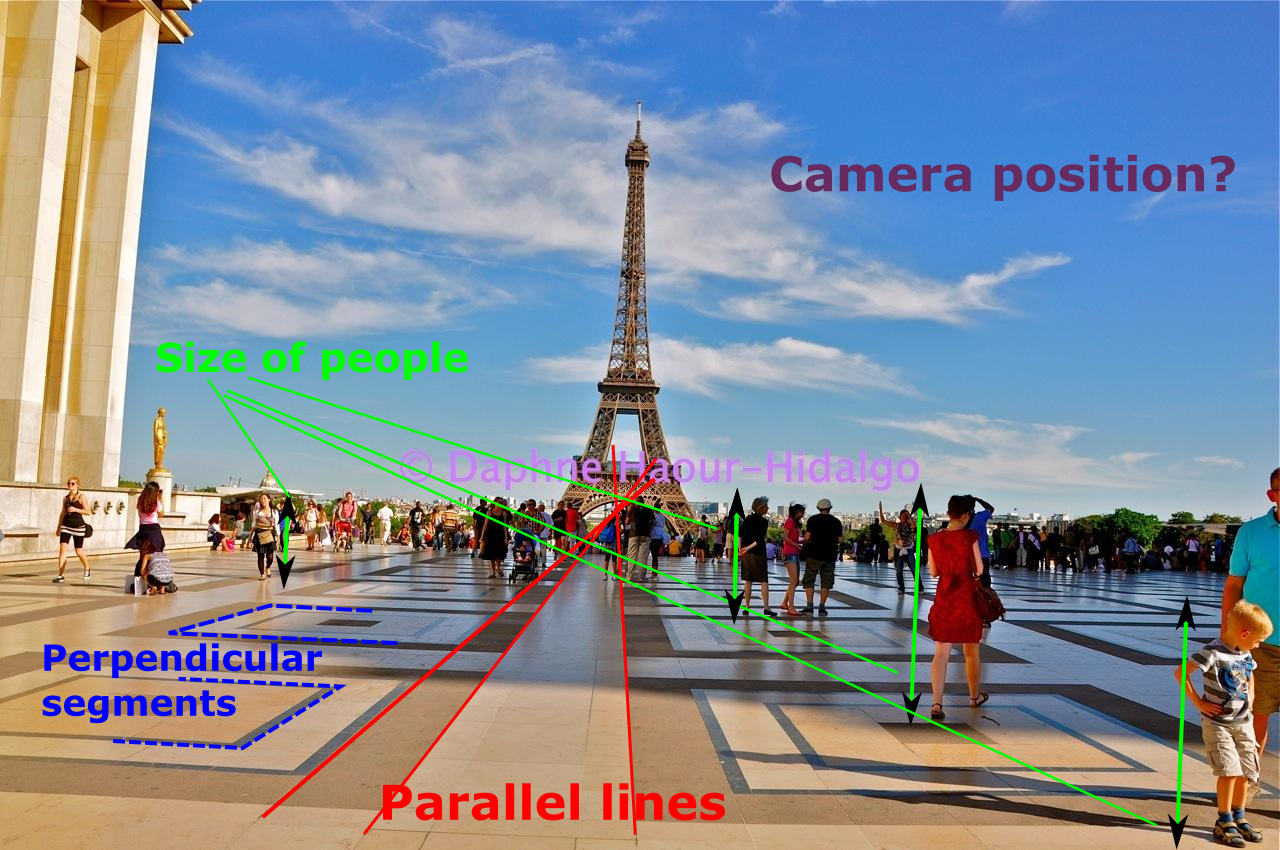
\includegraphics[width=\textwidth]{IMAGES/trocadero_annotations}
  \end{center}
\end{frame}


\begin{frame}
  \frametitle{Questions}
  Previous picture raises some questions about:\vfill
  \begin{itemize}
  \item Lines?
  \item Parallelism?
  \item Angles / orthogonality?
  \item Sizes?
  \item Camera position / Horizon?\vfill
  \end{itemize}
  What happens when you take a picture (or Daphn{\'e} Haour-Hidalgo in the previous case :-))
\end{frame}


\section{The Pinhole Camera}

\begin{frame}
  \frametitle{Getting an Image -- I}
  \begin{center}
    \includegraphics[width=0.55\textwidth]{FIGURES/oliphantnopinhole}
  \end{center}
  Many rays emanating from the same position touch the image sensitive
  array at many location: big blur!
\end{frame}


\begin{frame}
  \frametitle{Getting an Image -- II}
  \begin{center}
    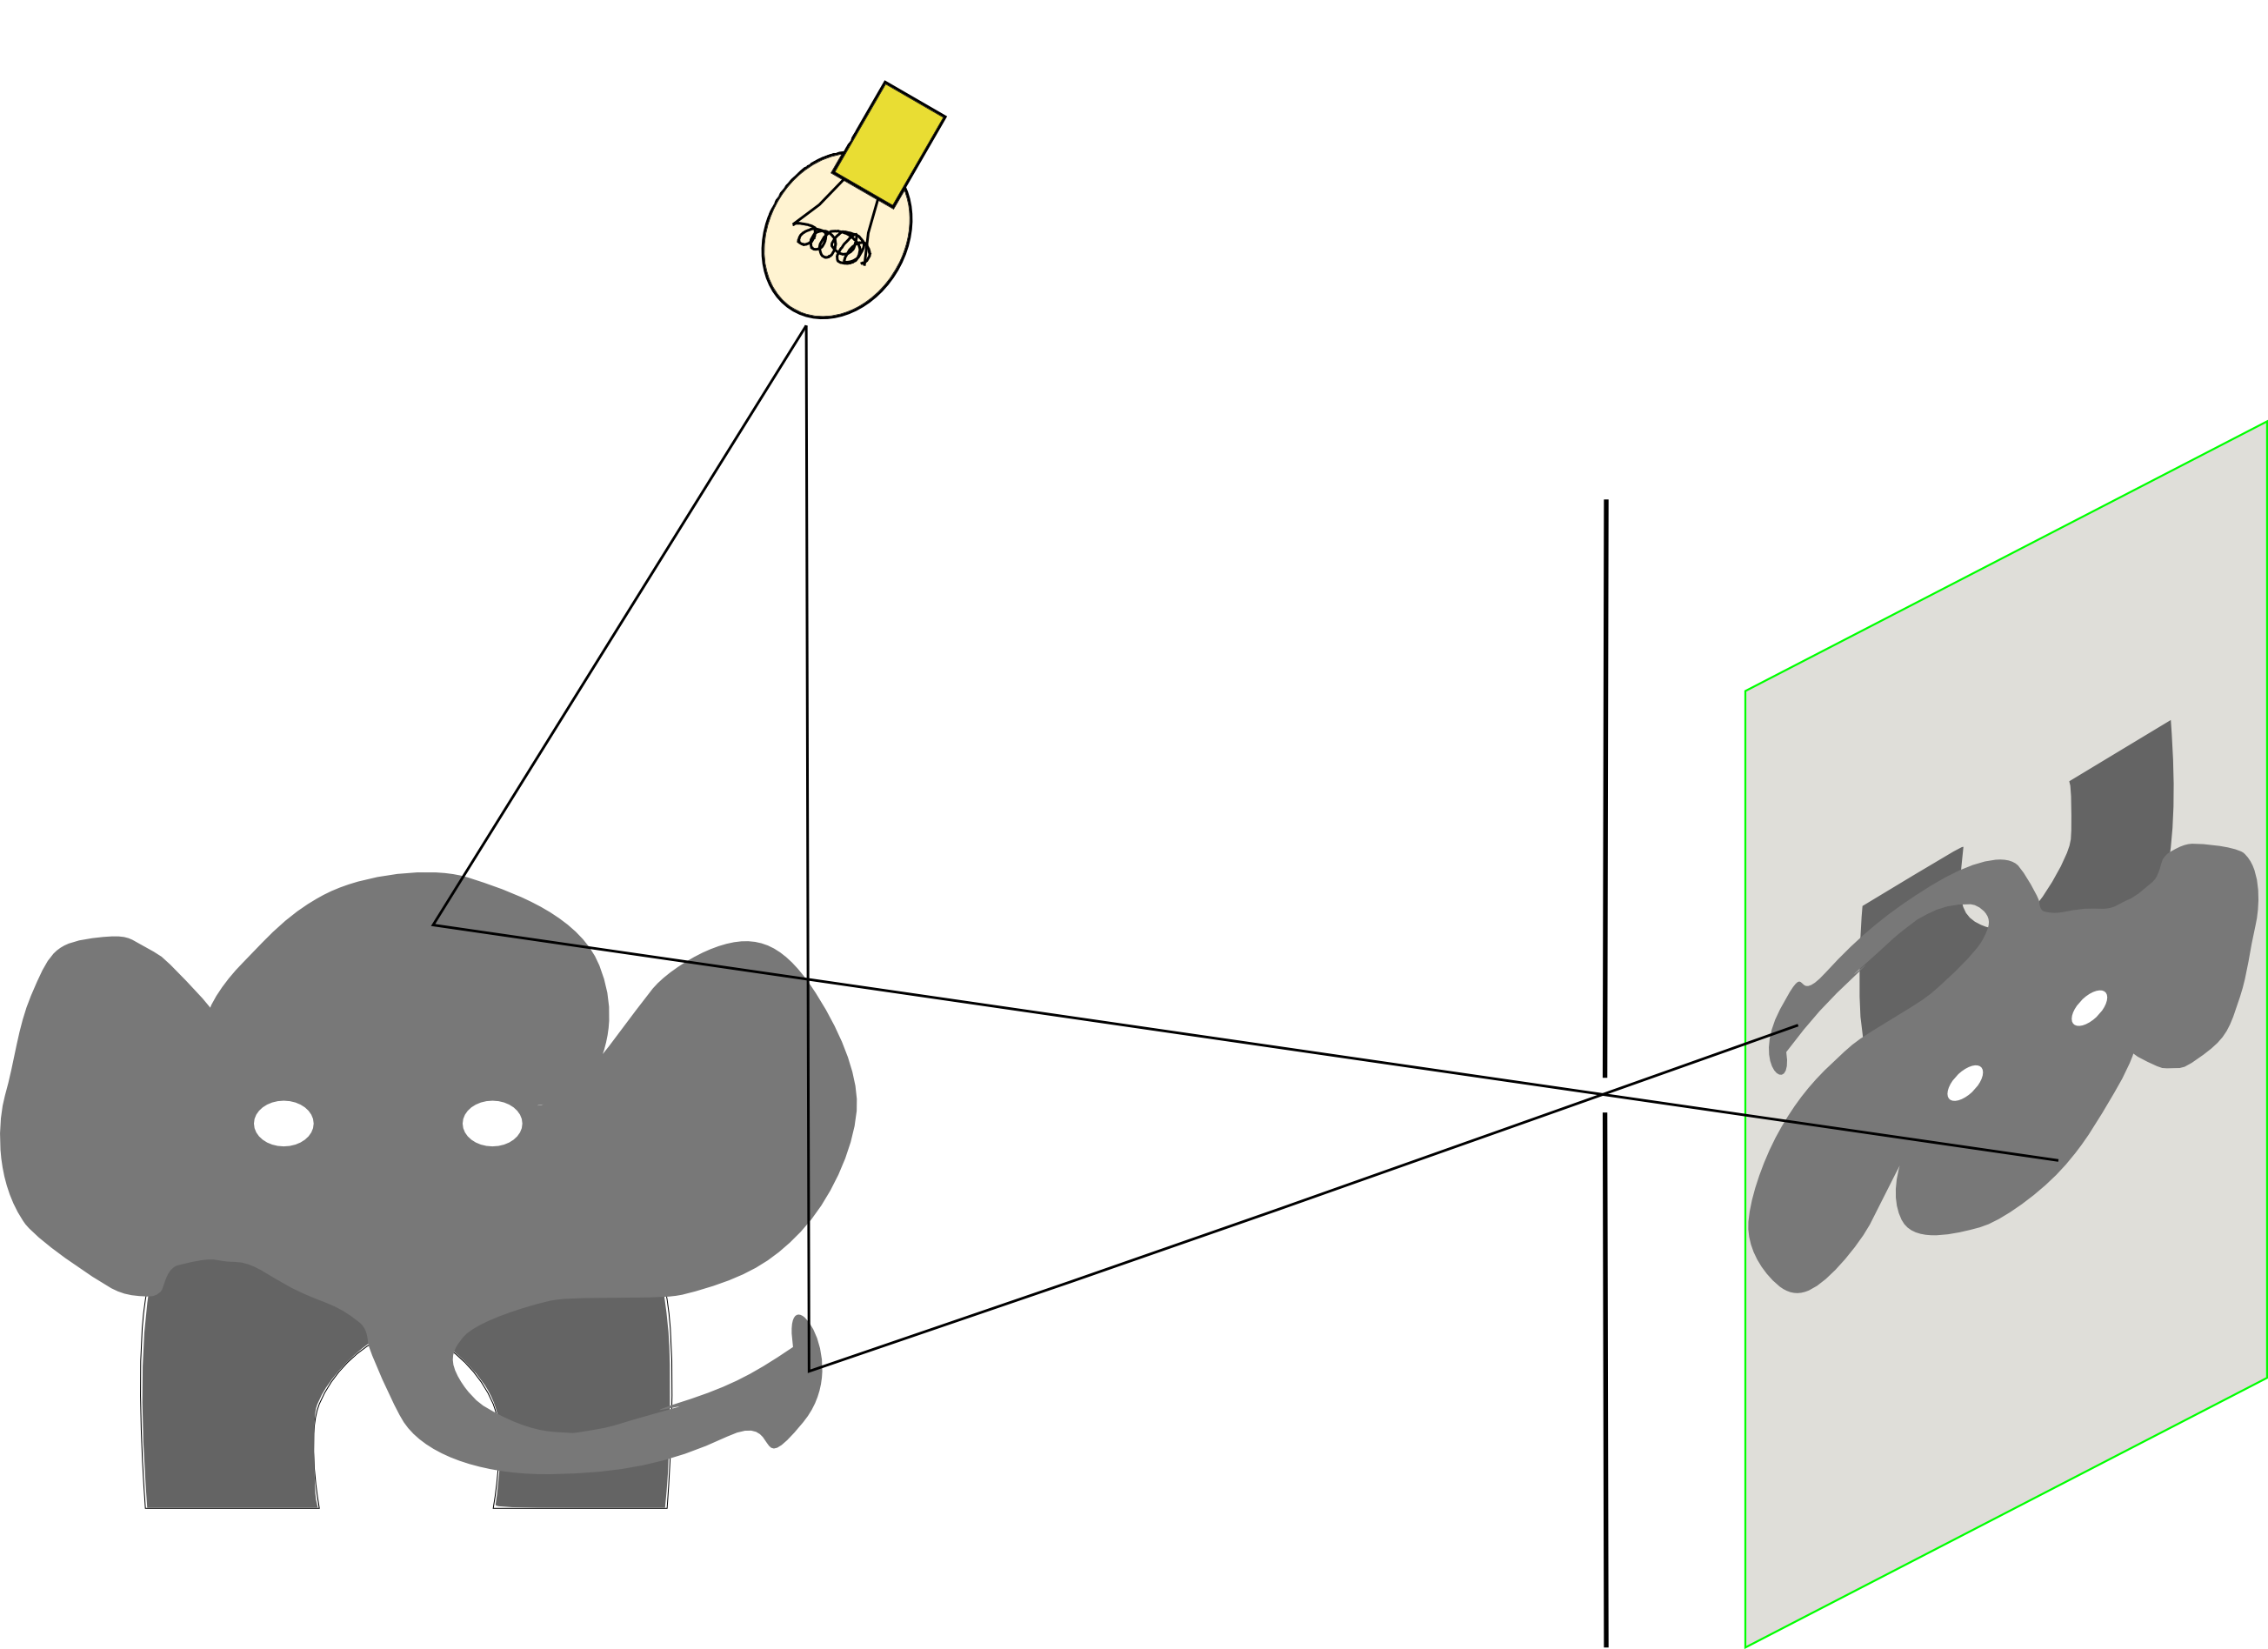
\includegraphics[width=0.65\textwidth]{FIGURES/oliphantpinhole}
  \end{center}
  Filtering the rays via a pinhole: get an (inverted) image. Principle
  of the \myemph{Camera Obscura} (dark room).
\end{frame}

\section{A bit of History}


\begin{frame}
  \frametitle{Camera Obscura}
  \begin{center}
    \begin{tabular}[h]{cc}
      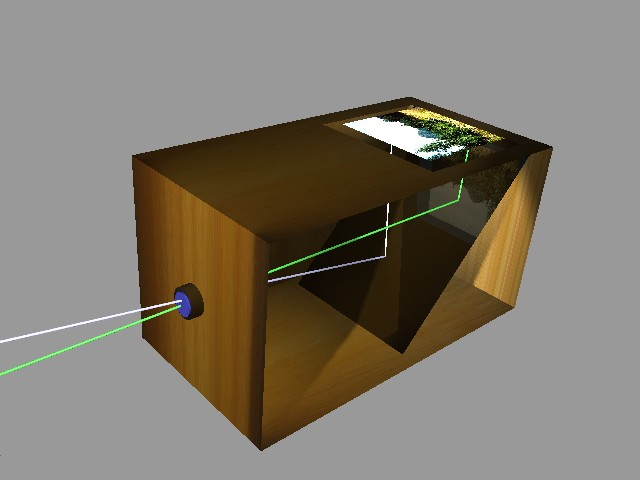
\includegraphics[width=0.4\textwidth]{IMAGES/WMCamera_obscura_box} &
      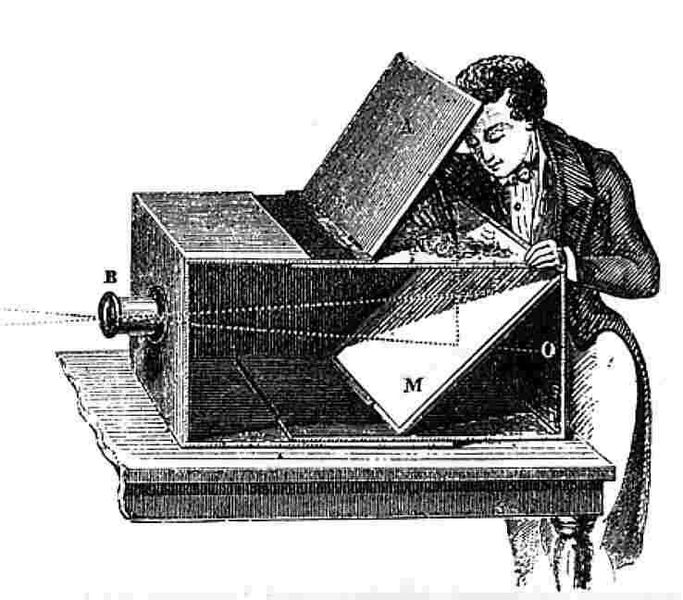
\includegraphics[width=0.4\textwidth]{IMAGES/WMCameraObscura18thCentury}\\
      Principle of Camera Obscura & 18th Century Camera Obscura
    \end{tabular}
  \end{center}
  \begin{itemize}
  \item Known from old chines writings
  \item Mentioned by Aristotle
  \item Plaque with photosensitive material: Photographic camera!
  \end{itemize}
\end{frame}

\begin{frame}
  \frametitle{The Very First Photography, 1826}
  \begin{center}
    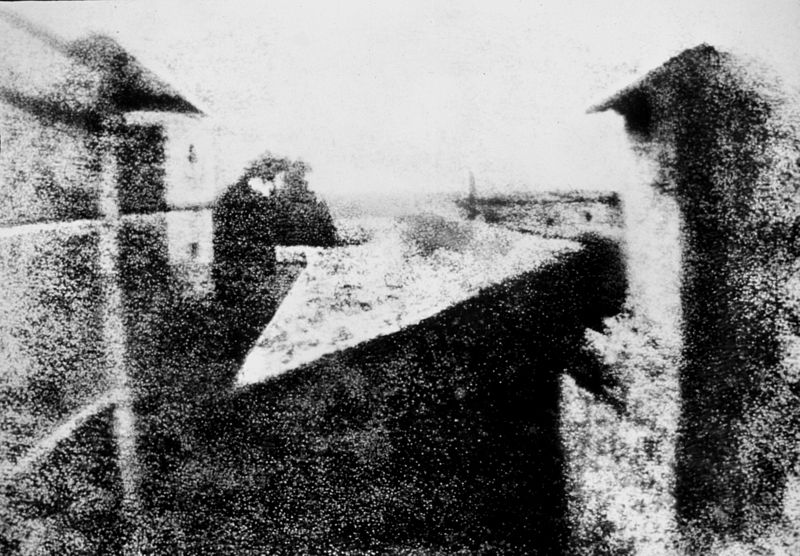
\includegraphics[width=0.8\textwidth]{IMAGES/WindowLegrasNiepce}\\
    
    {\fontsize{7}{8}\selectfont J. Nic{\'e}phore Ni{\`e}pce, View from the window at Le Gras,
      Saint Loup de Varennes, France -- Now at University of Texas at
      Austin.}
\end{center}
\end{frame}


\begin{frame}
  
  \begin{center}
    \frametitle{The Pioneers}
    \begin{tabular}[h]{ccc}
      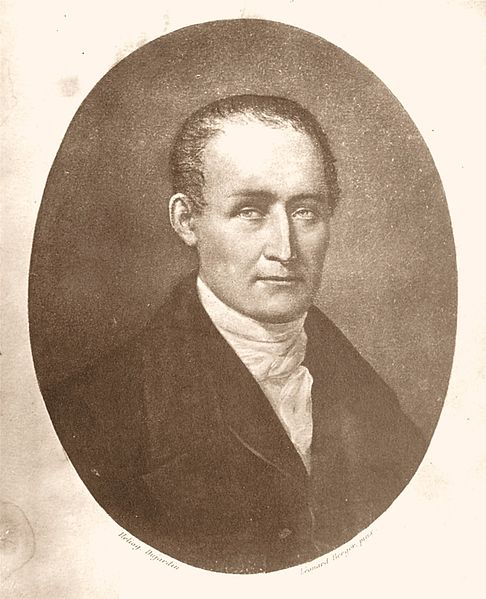
\includegraphics[width=0.3\textwidth]{IMAGES/JNNiepce} &
      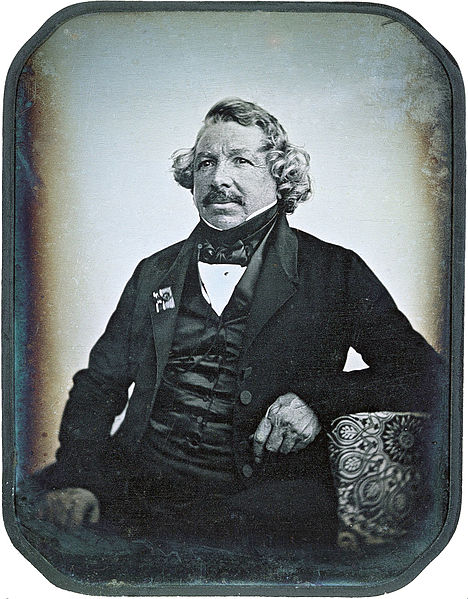
\includegraphics[width=0.3\textwidth]{IMAGES/LDaguerre} &
      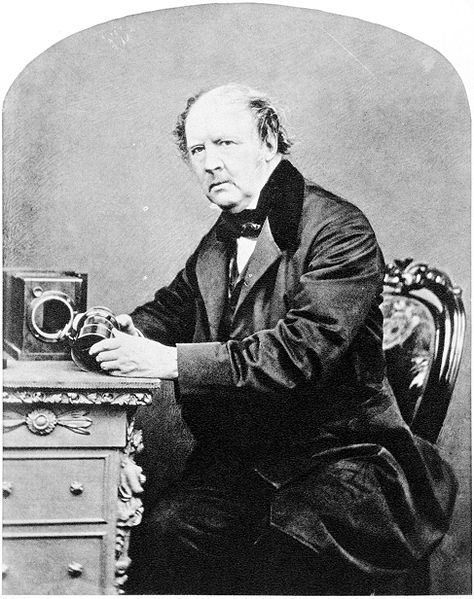
\includegraphics[width=0.3\textwidth]{IMAGES/HFTalbot} \\
      J. Nic{\'e}phore Ni{\`e}pce & Louis Daguerre & Henri F. Talbot
    \end{tabular}
  \end{center}
\end{frame}


\begin{frame}
  \frametitle{Now...}
  \begin{center}
    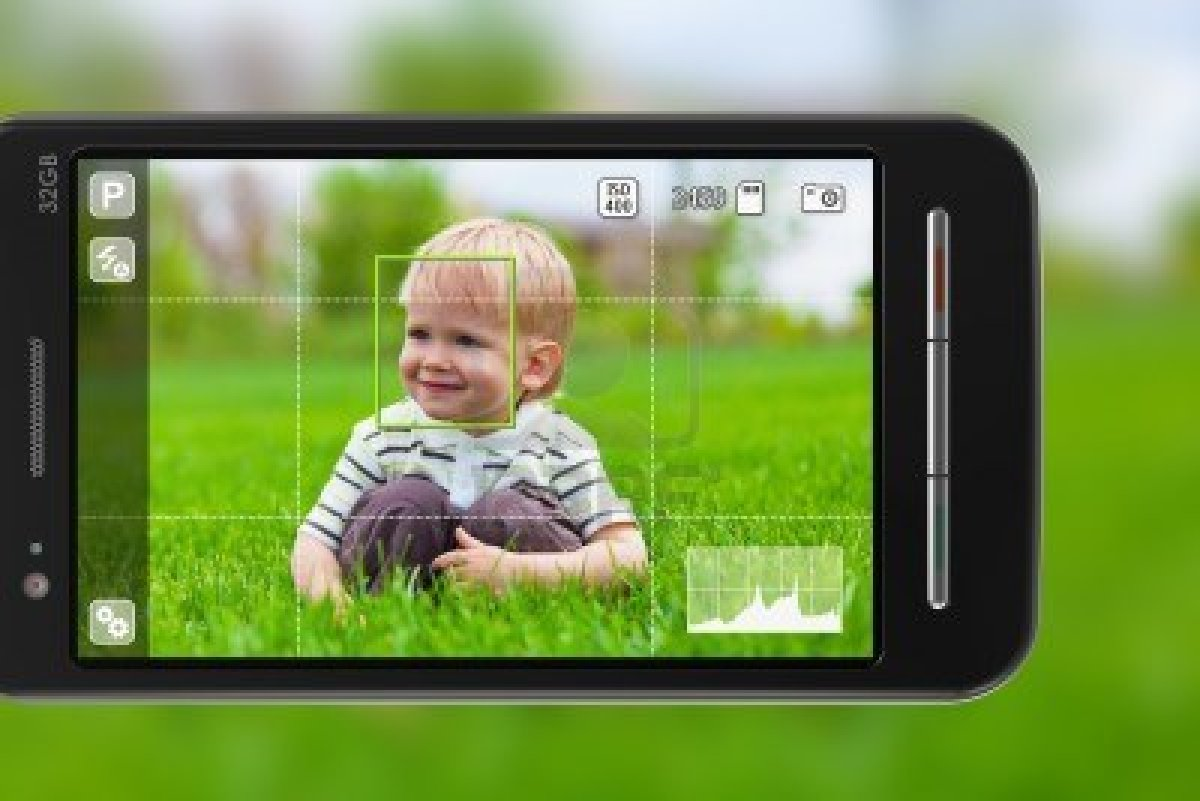
\includegraphics[width=0.8\textwidth]{IMAGES/smartphonecamera}
  \end{center}
\end{frame}



\section{Projection}


\begin{frame}
  \frametitle{The Pinhole Camera Model}
  \begin{center}
    \includegraphics[width=0.9\textwidth]{FIGURES/coproj}
  \end{center}
  \begin{itemize}
  \item $f$ is the focal length,
  \item $O$ is the camera center.
  \end{itemize}
\end{frame}


\begin{frame}
  \frametitle{Projection is Tricky!}
  \begin{center}
    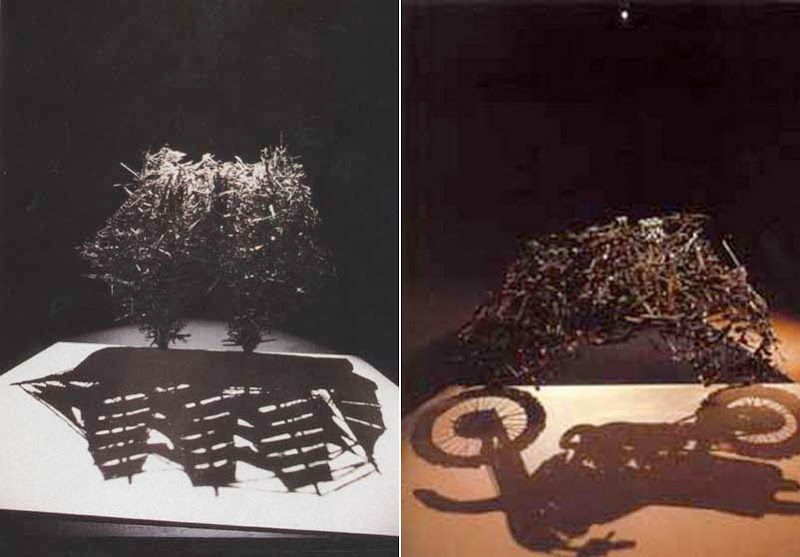
\includegraphics[width=0.8\textwidth]{IMAGES/shigeoFukuda}
  \end{center}
  Some illusions from Shigeo Fukuda. 
\end{frame}




% \begin{frame}
%   \frametitle{Perspective Effects}
%   Remember from Kim's first lecture
%   \begin{center}
%     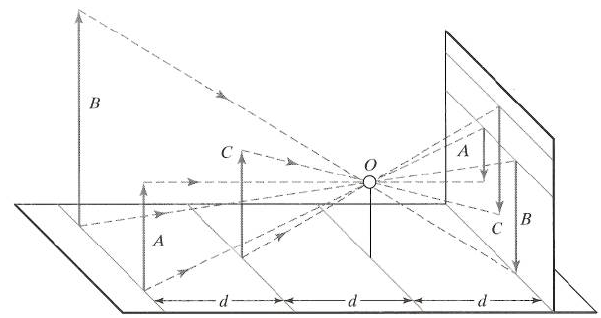
\includegraphics[width=0.9\textwidth]{FIGURES/fp131}
%   \end{center}
%   Far objects appear smaller that close ones.
% \end{frame}


% \begin{frame}
%   \frametitle{Perspective Effects}
%   Remember from Kim's first lecture again
%   \begin{center}
%     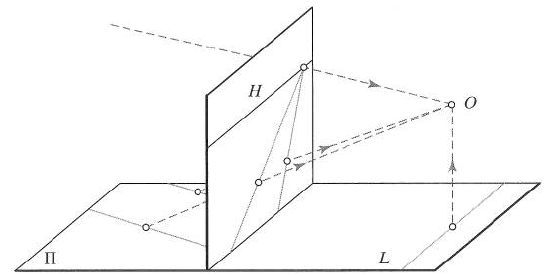
\includegraphics[width=0.9\textwidth]{FIGURES/fp132}
%   \end{center}
%   Images of parallel lines intersect at the horizon (virtual image plane).
% \end{frame}




\begin{frame}
  \frametitle{Lost in Projection and Preserved By Projection}
    \begin{center}
    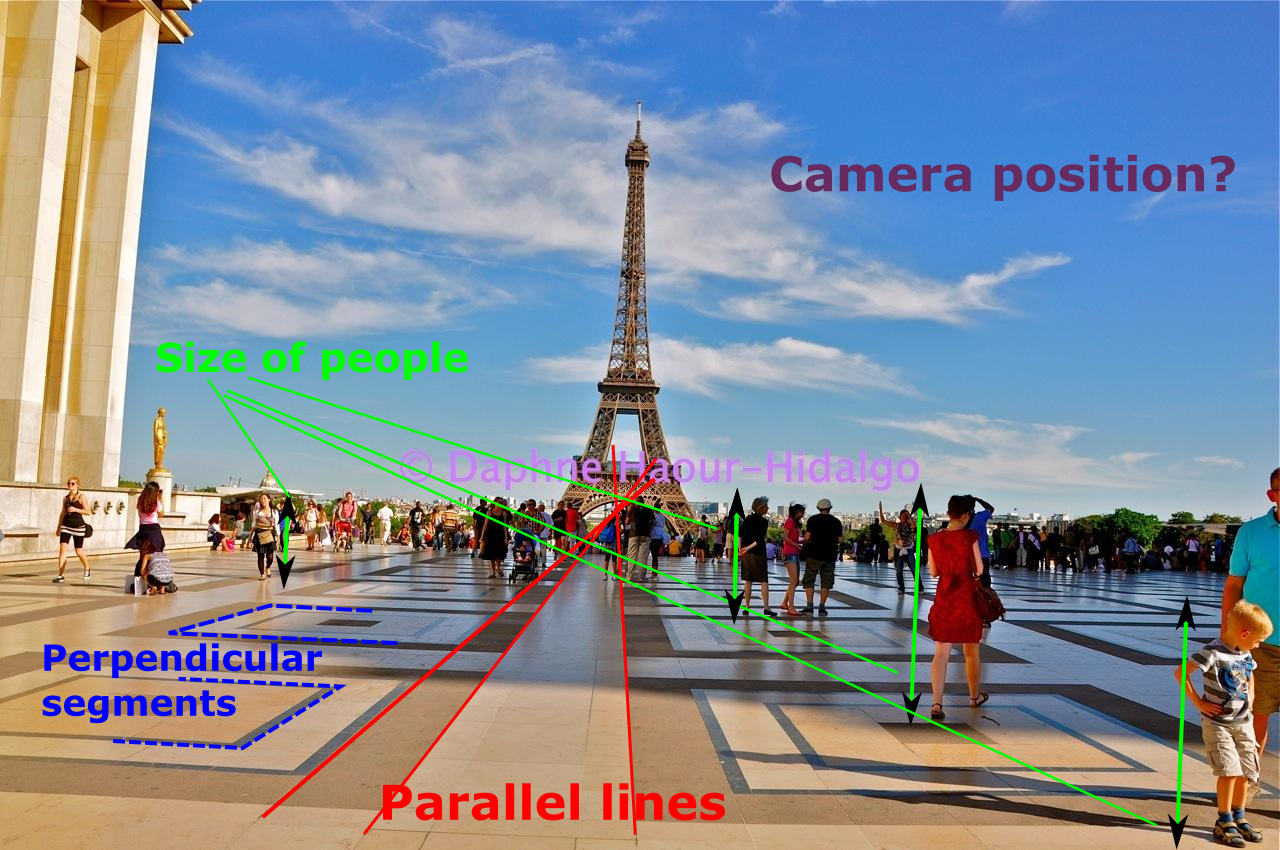
\includegraphics[width=0.8\textwidth]{IMAGES/trocadero_annotations}
  \end{center}
  More about than with S{\o}ren after New Year.
\end{frame}



\begin{frame}
  \frametitle{Projection Equations}
  \begin{center}
    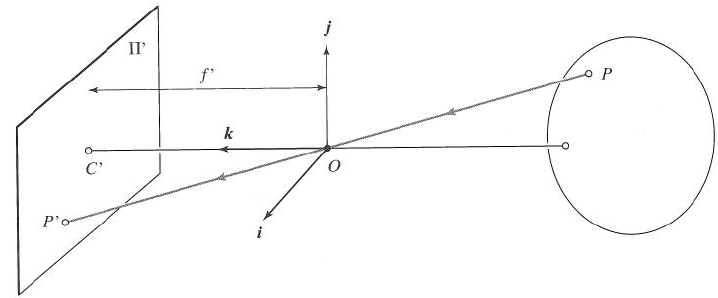
\includegraphics[width=0.6\textwidth]{FIGURES/fp14}
  \end{center}
  \begin{itemize}
  \item  $P (x,y,z)$, $P' (x',y',z')$. $P'$ in the image plane $\implies z' = f$.\\
    Thales a.k.a Similar Triangles Theorem:
   
  \end{itemize}
  \begin{columns}
    \begin{column}{0.5\textwidth}
    $$~~~~~~~~~
    \begin{bmatrix}x'\\
      y'
    \end{bmatrix}=
    \begin{bmatrix}
      f\dfrac{x}{z}\\~\\
      f\dfrac{y}{z}
    \end{bmatrix},\quad
    D_I//D_z
    $$   
    \end{column}
    \begin{column}{0.5\textwidth}
      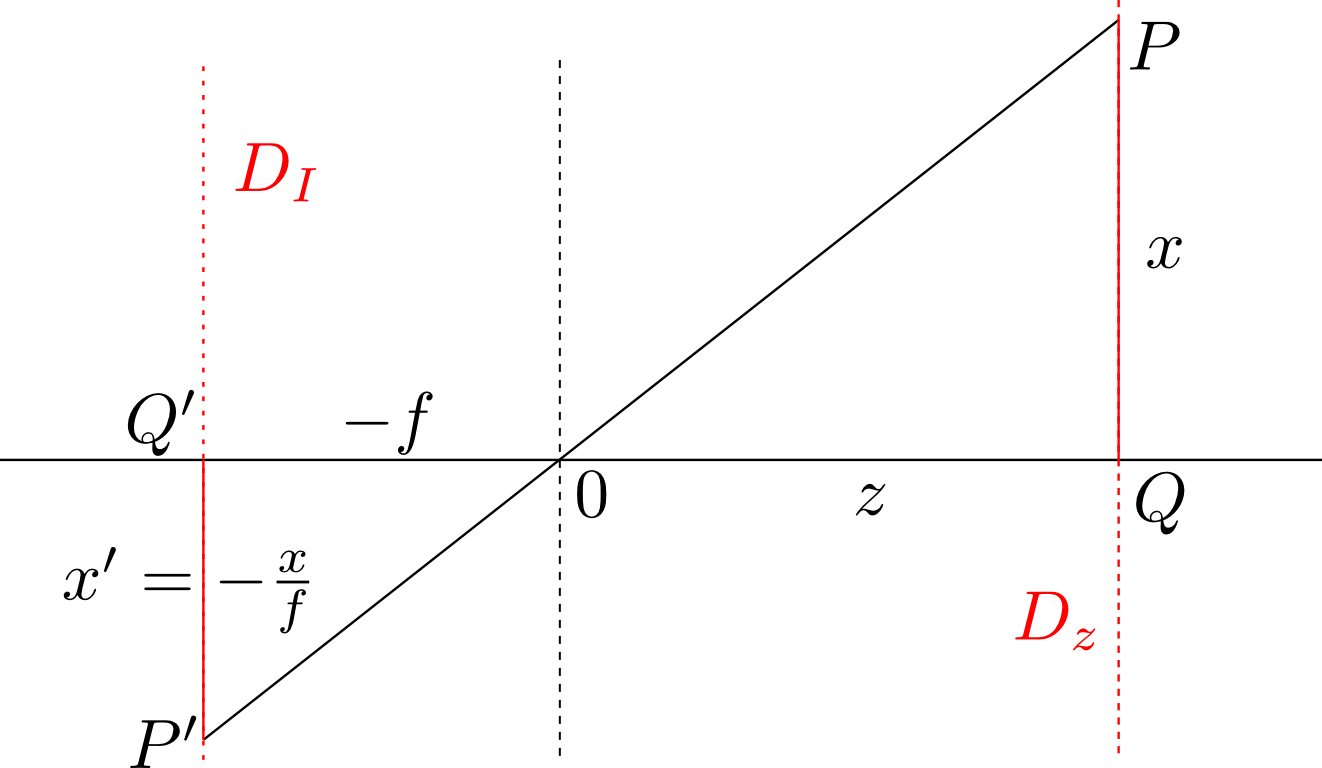
\includegraphics[width=1\textwidth]{FIGURES/thales_proj}
    \end{column}
  \end{columns}
\end{frame}

\begin{frame}[t]{Homogeneous Coordinates}
  \begin{itemize}
  \item Mapping $Pr:\begin{bmatrix}x \\ y \\ z\end{bmatrix} \mapsto\begin{bmatrix}f\frac{x}{z}\\f\frac{y}{z}\end{bmatrix}$ non linear but...
  \item Use \myemph{Homogeneous Coordinates}
    $$
    \left(a:b:c\right) =
      \begin{pmatrix}
        a\\b\\c
      \end{pmatrix}
      =
      \begin{bmatrix}
        \frac{a}{c}\\\frac{b}{c}
      \end{bmatrix}
    $$
    \item With them, $\begin{bmatrix}f\frac{x}{z}\\f\frac{y}{z}\end{bmatrix} =
      \begin{pmatrix}
        fx\\fy\\z
      \end{pmatrix}$, (Obs: [] and ()), 
      $$
      Pr=
      \begin{bmatrix}
        f & 0 & 0\\
        0 & f & 0\\
        0 & 0 & 1
      \end{bmatrix},\quad
      Pr
      \begin{pmatrix}
        \lambda a\\\lambda b\\\lambda c
      \end{pmatrix}
      =
      \begin{pmatrix}
        f \lambda a\\ f\lambda b\\\lambda c
      \end{pmatrix}
      =
      \begin{bmatrix}
        \dfrac{fa}{c}\\~\\\dfrac{fb}{c}
      \end{bmatrix}
      $$
  \end{itemize}
  
\end{frame}


% \begin{frame}
%   \frametitle{Preserved by projection}
%     \begin{center}
%     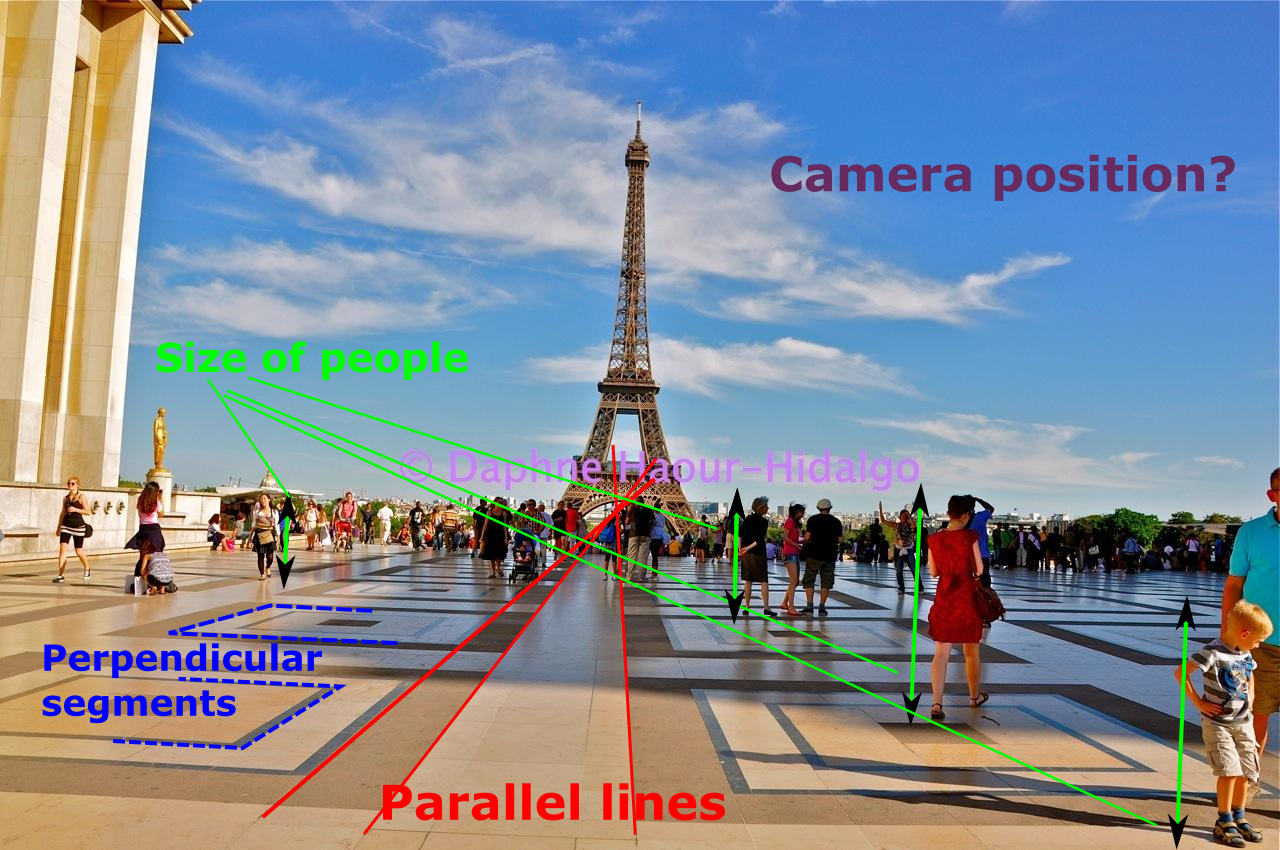
\includegraphics[width=0.8\textwidth]{IMAGES/trocadero_annotations}
%   \end{center}
%   Straight lines.
% \end{frame}

% \begin{frame}
%   \frametitle{Vanishing Points}
%     \begin{center}
%     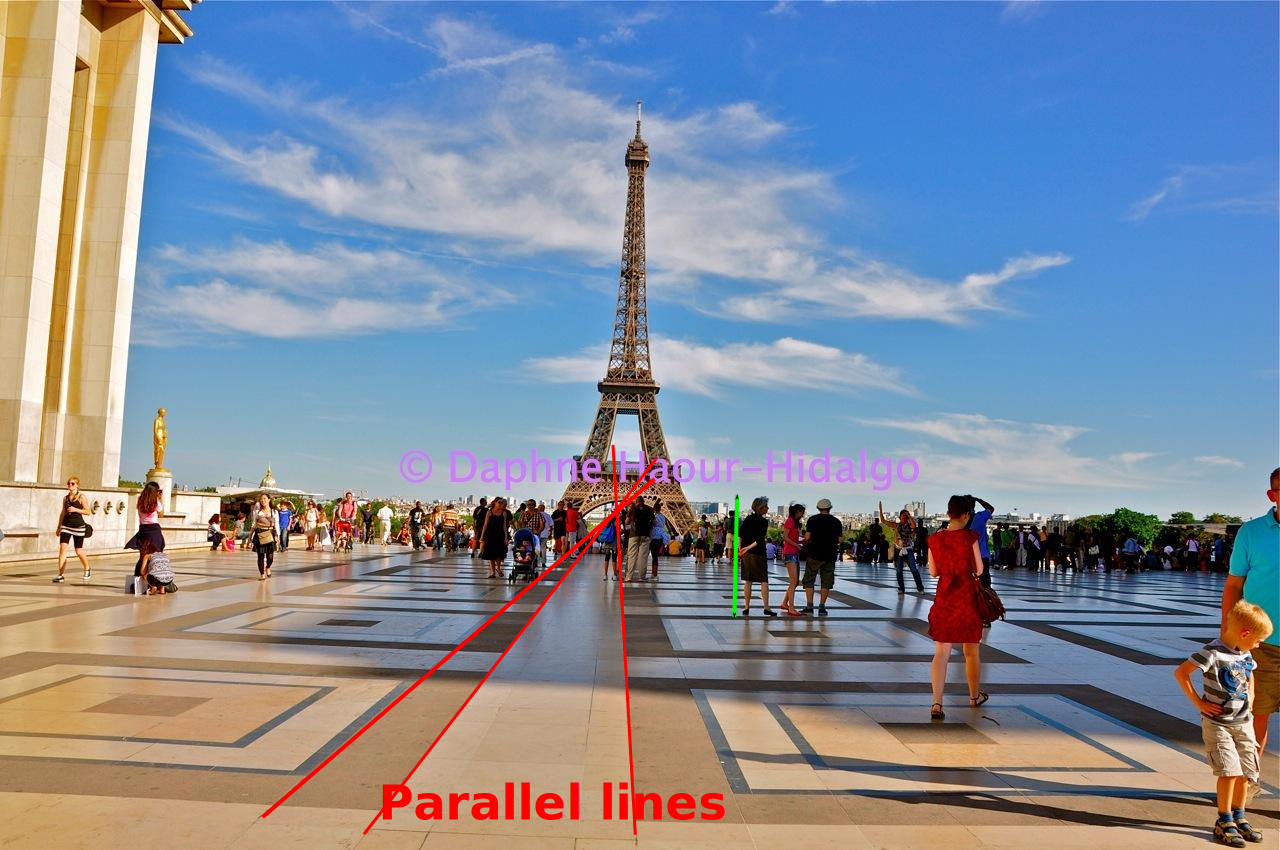
\includegraphics[width=0.8\textwidth]{IMAGES/trocaderolines}
%   \end{center}
%   Projections of parallel lines intersect at common points.
% \end{frame}

% \begin{frame}
%   \frametitle{Vanishing line}
%   \begin{center}
%     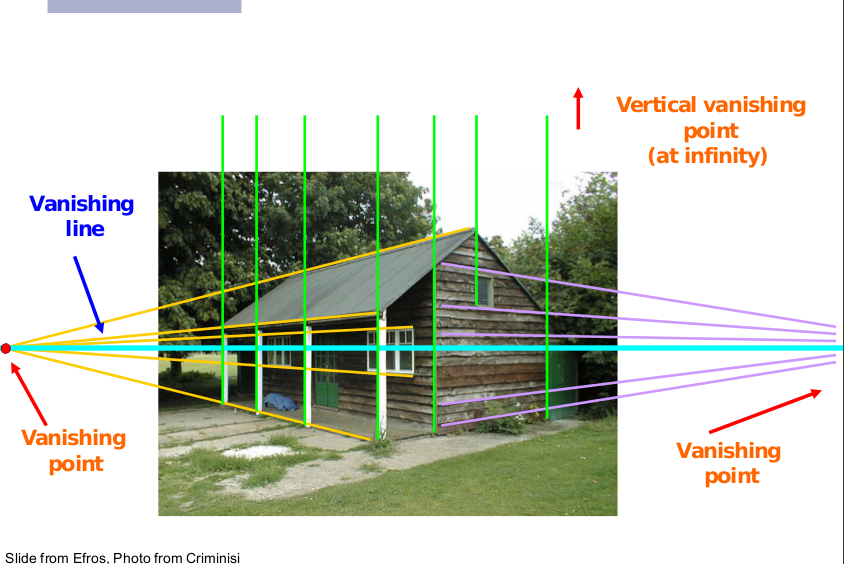
\includegraphics[width=0.7\textwidth]{FIGURES/vanishingline}
%   \end{center}
%   Vanishing points intersect at a common line. Intersection can be at infinity.
% \end{frame}

\begin{frame}
  \frametitle{Projective Line}
  \begin{itemize}
  \item In 1D: standard  coordinate = 1 number. 
    \begin{center}
      
\includegraphics[width=0.70\textwidth]{FIGURES/1dcoords}
    \end{center}
  \item Change of coordinates:
    $x\sim
    \begin{pmatrix}
      x\\1
    \end{pmatrix},\quad
    \begin{pmatrix}
      x\\w
    \end{pmatrix}\sim x/w 
    $
  \item ``Tame'' infinity! Point $P_\infty = (x,0)^T \sim x/0 = \pm\infty \sim (\pm\infty,1)^\top$.
    \begin{center}
      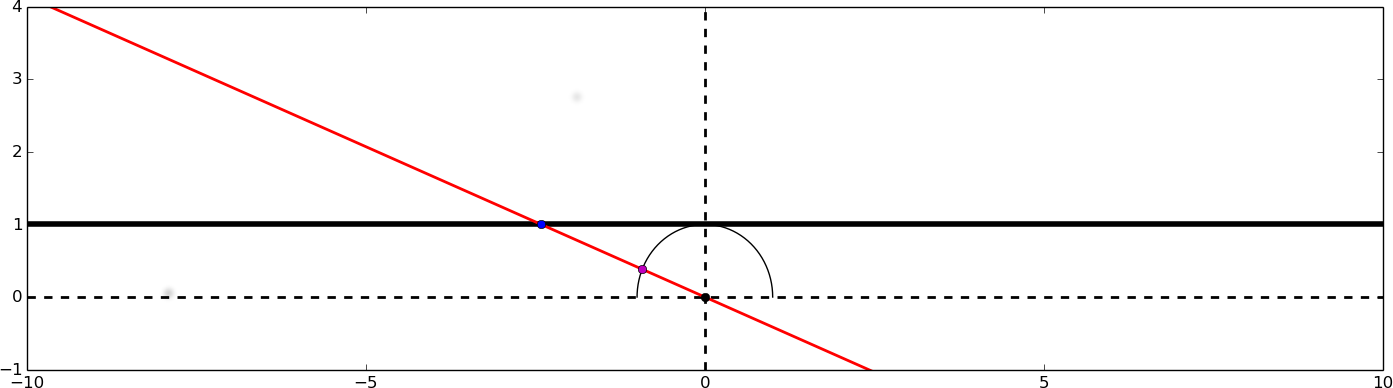
\includegraphics[width=0.5\textwidth]{FIGURES/proj050}\\
      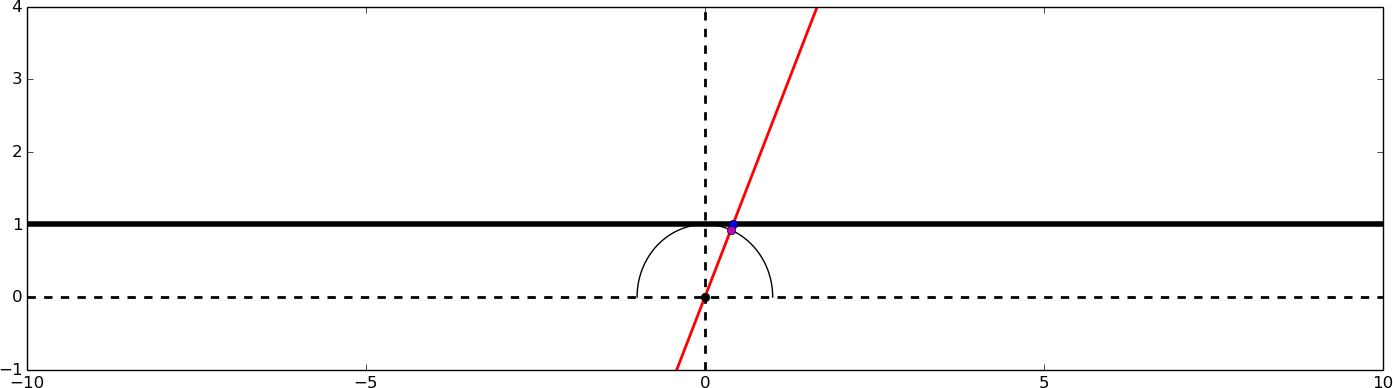
\includegraphics[width=0.5\textwidth]{FIGURES/proj250}~
      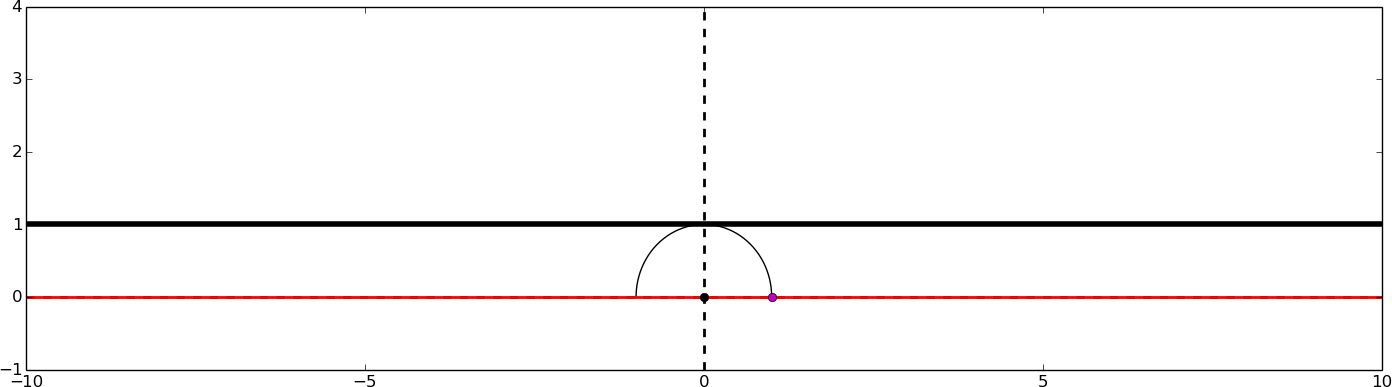
\includegraphics[width=0.5\textwidth]{FIGURES/proj400}\\
      Negative coordinate,
      positive coordinate, $\infty$ coordinate.
    \end{center}
  \item Usual line + $P_\infty$ = \myemph{Projective Line $\PP^1$} and $P_\infty$ = \myemph{Point at Infinity}
  \end{itemize}
\end{frame}


\begin{frame}[t]{1D homography}
  \begin{itemize}
  \item \myemph{Homography}: Isomorphic (1-to-1) transformation of projective line onto itself. 
  \item Written as 2x2 matrix $H$ with $\det(H)\not=0$.   
    $$
    H =
    \begin{pmatrix}
      a & b\\ c & d
    \end{pmatrix},\quad 
    \begin{pmatrix}
      a & b\\ c & d
    \end{pmatrix}
    \begin{pmatrix}
      x\\y
    \end{pmatrix}
    =
    \begin{pmatrix}
      ax + by\\cx + dy
    \end{pmatrix}\sim
    \frac{ax + by }{cx + dy}
    $$
  \item Linear mapping on line: multiplication by scalar $a$. Can be written
    $$
    \begin{pmatrix}
      a & 0\\ 0 &1
    \end{pmatrix}
    \begin{pmatrix}
      x \\ 1
    \end{pmatrix}
    =
    \begin{pmatrix}
      ax \\ 1
    \end{pmatrix}\sim ax.
    $$
    Special type of homography
  \item Linear mappings conserve distance ratios:
    \begin{columns}
      \begin{column}{0.6\textwidth}
        \flushright{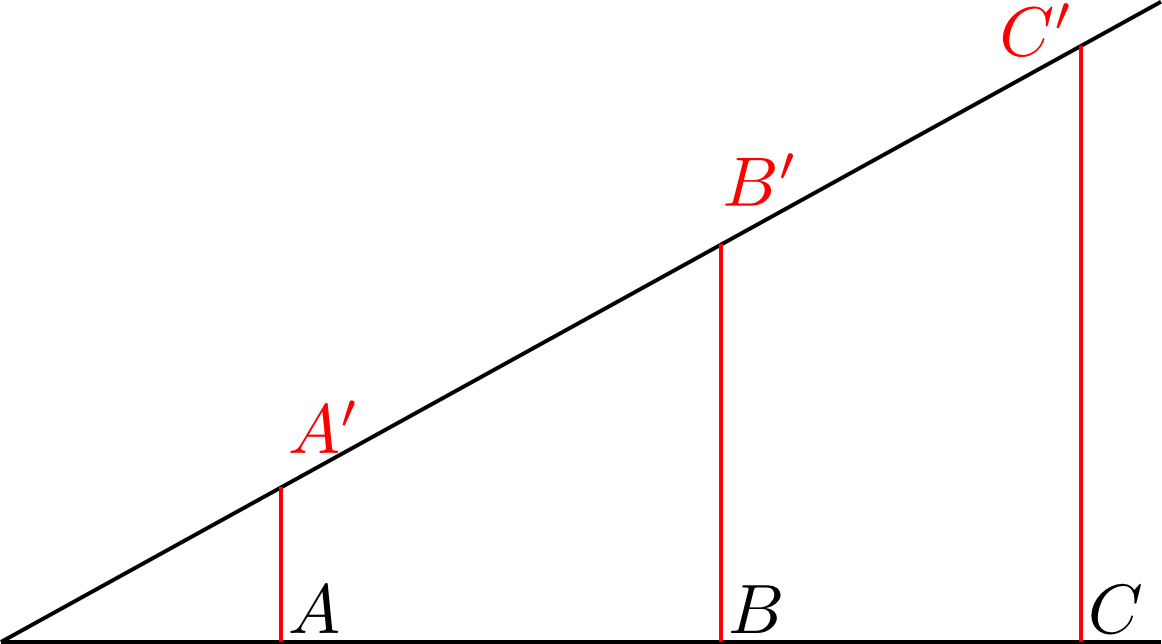
\includegraphics[width=0.8\textwidth, height=0.25\textheight]{FIGURES/linearratio}}
      \end{column}
      \begin{column}{0.4\textwidth}
        $$
        \frac{A'B'}{A'C'} = \frac{AB}{AC}
        $$
      \end{column}
    \end{columns}
  \end{itemize}
\end{frame}


\begin{frame}[t]{Cross-Ratio}
  \begin{itemize}
  \item Cross-Ratio of 4 points $A$, $B$, $C$ and $D$:
    $$
    (A;B;C;D) = \frac{AC\cdot BD}{BC\cdot AD}
    $$
  \item Geometric Representation of Homography
    \begin{center}
      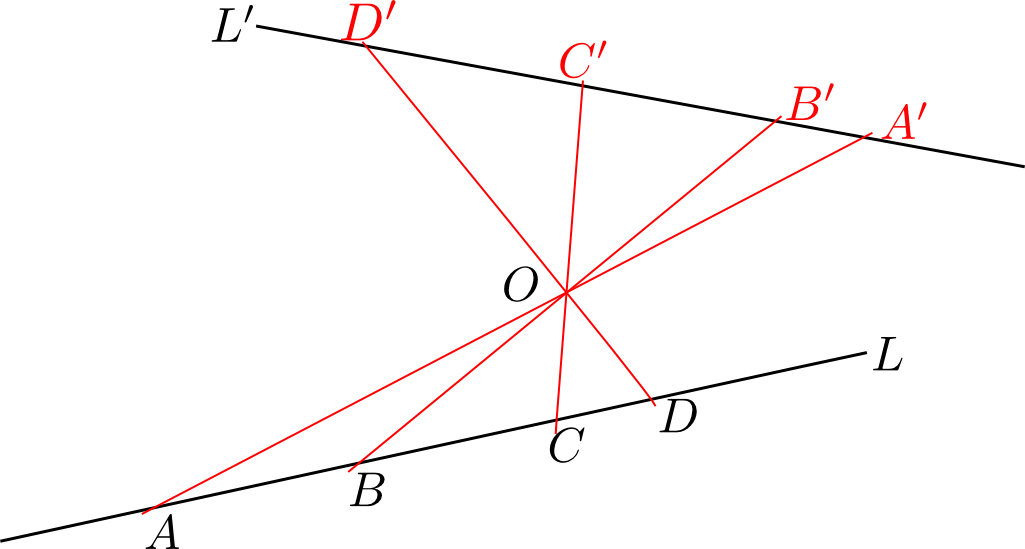
\includegraphics[width=0.6\textwidth]{FIGURES/crossratio}
    \end{center}
  \item $O$ would be camera optical center, Line $L$ in 3-space
    and line $L'$ in camera plane. Transformation from $L$ to $L'$: 1D homography. 
  \item Homographies conserve Cross-Ratio
    $$
    (A;B;C;D) = (A';B';C';D') = \frac{A'C'\cdot B'D'}{B'C'\cdot A'D'}
    $$
  \end{itemize}
  
\end{frame}

\begin{frame}[t]{Projective Geometry}
  \begin{itemize}
  \item Invented by artists, Late middle age.
  \item First formalization by Desargues (1591--1661).
  \item Idea: complete the line, plan, space with ``things'' at infinity and make infinity ``close''.
  \end{itemize}
  Homogeneous Coordinates.
  \begin{itemize}
  \item Add an extra coordinate!
  \item in Plan $[x,y]\sim (x,y,1)$, $(x,y,z)\sim [x/z,y/z]$, $z\not=0$.
  \item Planar Line equation, Projective planar line equation 
    $$
    \text{Euclidean: } ax + by + c = 0,\quad \text{Projective: } ax + by + cz = 0.
    $$
  \item Parallel lines in Euclidean Plan:
    $$
    \begin{cases}
      L_1: &ax + by + c = 0\\
      L_2: &ax + by + d = 0
    \end{cases},\quad
    L_1\cap L_2 = \emptyset
    $$
  \end{itemize}
\end{frame}

\begin{frame}[t]{Parallel lines in Projective Space?}
  $$   \begin{cases}
      L_1: &ax + by + cz = 0\\
      L_2: &ax + by + dz = 0
    \end{cases},\quad
    L_1\cap L_2 = 
    \begin{cases}
      &ax + by = 0\\
      &\fbox{z = 0}
    \end{cases}
  $$
  \begin{center}
    \includegraphics[width=0.7\textwidth]{FIGURES/parallel_lines_p2}~\\
    ~\\
     $z=0$ means ``in the extra stuff at infinity''!
  \end{center}
 ~\\
  {\fontsize{6}{6}\selectfont
    \begin{itemize}
    \item Exercise: $P$ with coordinates $(x,y,1)$. $Q(x',y',w)$ point
      on the line through $O (0,0,0)$ and $P$.  Compute $x'$ and $y'$.
      Considering $[x',y',w]$ as homogeneous 2D coordinates, what are
      the corresponding 2D coordinates?
    \end{itemize}
  }
\end{frame}



\begin{frame}[t]{Projective Plane and Camera}
  \begin{center}
  \begin{tabular}[h]{cc}
    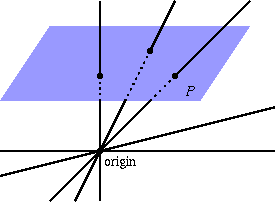
\includegraphics[width=0.4\textwidth]{FIGURES/2dprojspace} &
    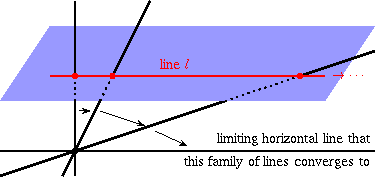
\includegraphics[width=0.4\textwidth]{FIGURES/pointsinfty}
  \end{tabular}
  \end{center}
  \begin{columns}
    \begin{column}{0.4\textwidth}
      $z = 1$ and $z = -f$
    \end{column}
    \begin{column}{0.6\textwidth}
      
\includegraphics[width=1\textwidth]{FIGURES/projcoords1}
    \end{column}
  \end{columns}
\end{frame}


\begin{frame}[t]{Homography in 2D}
  \begin{itemize}
  \item Isomorphism of the projective plane
  \item Maps lines to lines.
  \item Can be represented by a (non-unique) $3x3$ invertible matrix (Non zero determinant).
    $$
    H \sim
    \begin{pmatrix}
      a & b & c\\
      d & e & f\\
      g & h & i
    \end{pmatrix}\sim
    \begin{pmatrix}
      \lambda a & \lambda b & \lambda c\\
      \lambda d & \lambda e & \lambda f\\
      \lambda g & \lambda h & \lambda i
    \end{pmatrix}
    $$
  \item Standard vector $[x,y]\sim (x,y,1)^T$. If $i\not=0$ in $H$: divide all terms by $i$: $a \leftarrow a/i$, $b\leftarrow b/i\dots$
    $$
    \begin{pmatrix}
      \lambda a & \lambda b & \lambda c\\
      \lambda d & \lambda e & \lambda f\\
      \lambda g & \lambda h & \lambda 1
    \end{pmatrix}
    \begin{pmatrix}
     x \\y\\1
    \end{pmatrix}
    =
    \begin{pmatrix}
      x'\\y'\\z'
    \end{pmatrix}
    $$
  \item No guaranty that $z'\not=0$: Can send a point to infinity. 
  \end{itemize}
\end{frame}


\begin{frame}[t]{Example of 2D Homography}
  Matrix of homography is 
  $$
  H =
  \begin{pmatrix}
    2\cos\theta& -\sin\theta& -\frac32\\
    \sin\theta&  \cos\theta& -\frac32\\
    \frac12 & 0 & \frac12
  \end{pmatrix},\quad \theta = 1.02.
  $$
  \begin{center}
    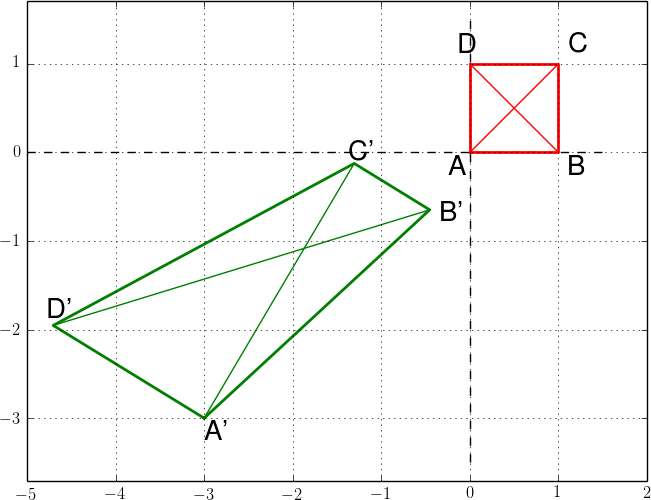
\includegraphics[width=0.6\textwidth]{FIGURES/python2dhomog.png}
  \end{center}
\end{frame}


\begin{frame}[t]{Homographies in Computer Vision}
  \begin{center}
    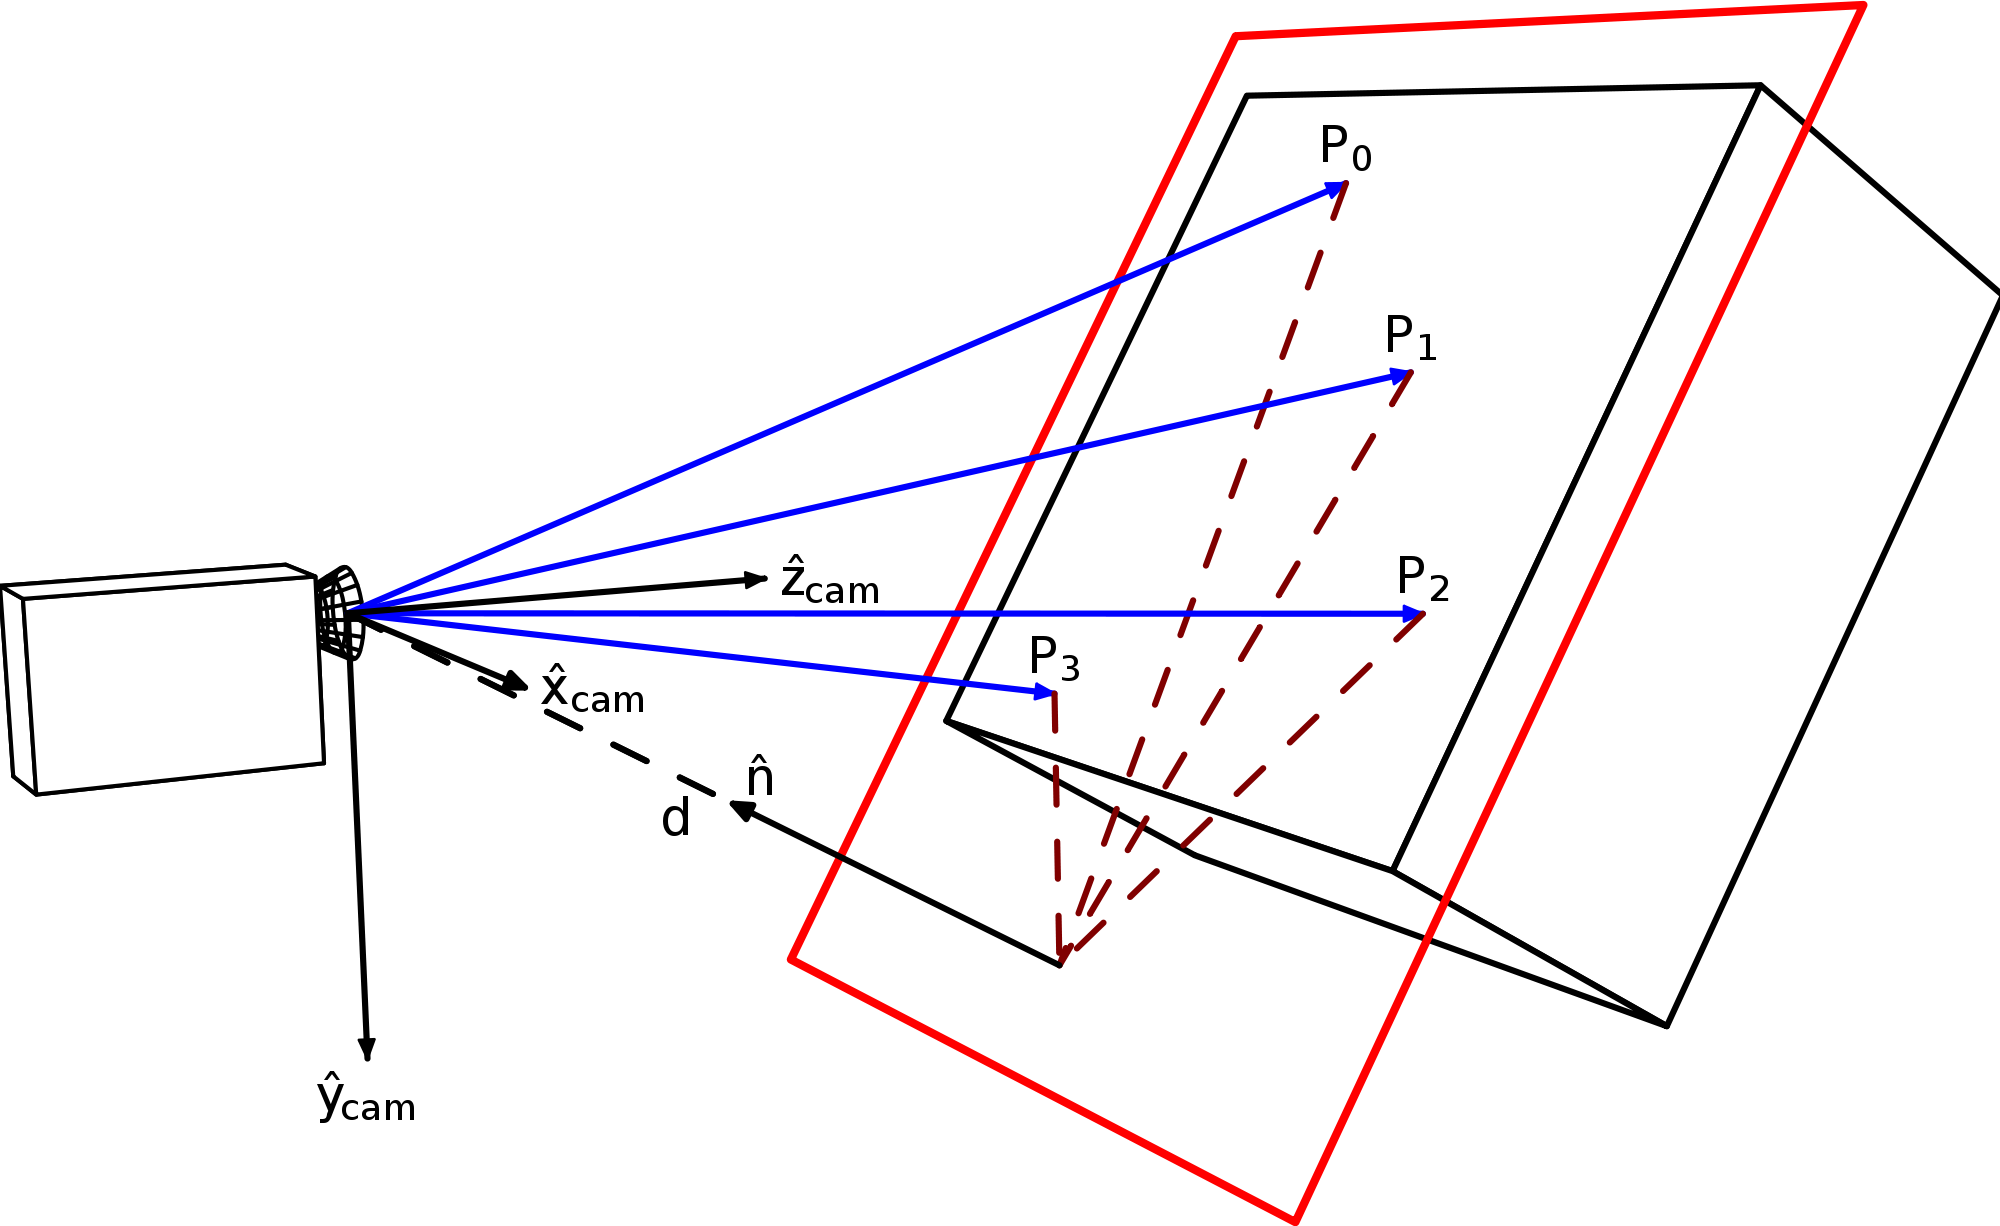
\includegraphics[width=0.5\textwidth]{FIGURES/Homography_wikipedia}\\
    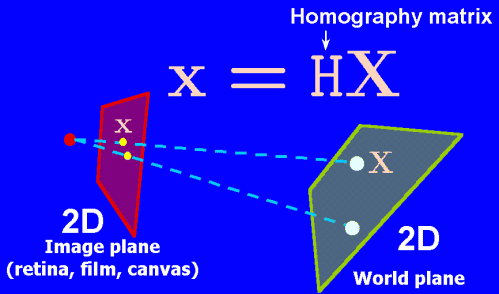
\includegraphics[width=0.5\textwidth]{FIGURES/homographyplusmathorg}
  \end{center}
\end{frame}



\begin{frame}
  \frametitle{Homogeneous coordinates, 3D}
  \begin{itemize}
  \item From 3D point coordinate to 3D Homogeneous coordinate
    $$
    (x,y,z)\Implies
    \begin{bmatrix}
      x\\y\\z\\1
    \end{bmatrix}
    $$
  \item From 3D homogeneous coordinates to 3D coordinates
    $$   
    \begin{bmatrix}
      x\\y\\z\\w
    \end{bmatrix}
    \Implies 
    (x/w, y/w, z/w)
    $$
  \end{itemize}
\end{frame}

\begin{frame}[t]{Homographies}
  Matrix known \emph{up to a scalar}.
  \begin{itemize}
  \item Contains Linear mappings and translations for points not at $\infty$.
  \item $2D$ linear mapping as homography
    $$
    A =
    \begin{bmatrix}
      a & b\\
      c & d
    \end{bmatrix},\quad
    H_A =
    \begin{pmatrix}
      a & b & 0\\
      c & d & 0\\
      0 & 0 & 1
    \end{pmatrix}
    $$
    \item Translation by vector $v = [v_x, v_y]$ as homography:
      $$
      H_v =
      \begin{pmatrix}
        1 & 0 & v_x\\
        0 & 1 & v_y\\
        0 & 0 & 1
        
      \end{pmatrix}
      $$
  \end{itemize}
\end{frame}


% \begin{frame}
%   \frametitle{Homogeneous coordinates}
%   \begin{center}
%     
\includegraphics[width=0.7\textwidth]{FIGURES/projcoords1}
%   \end{center}
%   Homogeneous coordinates in 2D correspond to points in plane $z=1$
%   but also to lines through the origin and this point.
% \end{frame}

\begin{frame}
  \frametitle{Why Are They Useful}
  \begin{itemize}
  \item Projection to image plane in standard coordinates:
    $$
    P: (x,y,z)\mapsto P': (f\frac{x}{z}, f\frac{y}{z})
    $$
  \item In homogeneous coordinates:\pause
    $$
    P:
    \begin{bmatrix}
      x\\y\\z\\1
    \end{bmatrix}
    \mapsto P': 
    \begin{bmatrix}
      fx\\fy\\z
    \end{bmatrix}
    $$
  \item Matrix notation
    $$
     \begin{bmatrix}
      fx\\fy\\z
    \end{bmatrix}
    = \udesc{M}{
    \begin{bmatrix}
      f & 0 & 0 & 0\\
      0 & f & 0 & 0\\
      0 & 0 & 1 & 0
    \end{bmatrix}}
    \begin{bmatrix}
      x\\y\\z\\1
    \end{bmatrix}
    $$
    \item $M$ is the \myemph{Camera Matrix}
  \end{itemize}
\end{frame}


\begin{frame}
  \frametitle{World,Camera and Image Coordinates}
  In the previous slides, Many coordinate systems are implicitly known:
  \begin{itemize}
  \item 3D World Coordinates: Coordinate system of the 3D world.
  \item Camera Coordinates: 3D coordinate system attached to the camera.
  \item Image Coordinates: 2D Coordinate system attached to the image plane.
  \end{itemize}
  Not that simple in practice! S{\o}ren After New Year!
\end{frame}

% \begin{frame}
%   \frametitle{Assumptions Behind the Simple Model}
%   \begin{center}
%     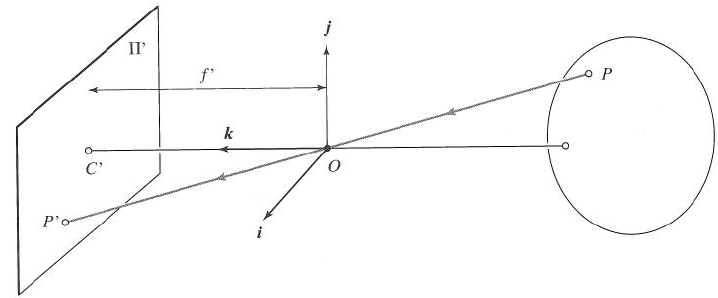
\includegraphics[width=0.9\textwidth]{FIGURES/fp14}
%   \end{center}
%   \begin{itemize}
%     \item The camera center $0$ is the same as the world coordinates origin,
%     \item The axes $\bi$, $\bj$ and $\bk$ are common for the camera and the world
%     \item Pixels are squared and perfectly aligned with the camera coordinates.
%     \item Image coordinates have their origin at $C'$, projection of the camera center $O$.
%   \end{itemize}
% \end{frame}


% \begin{frame}
%   \frametitle{Intrinsic vs Extrinsic Camera Parameters}
%   Intrinsic parameters refer to internal parameters:
%   \begin{itemize}
%   \item Position of the image center writ projection of the camera center: 2 parameters
%   \item Scale factors for the pixels sizes in both x and y directions: 2 parameters,
%   \item Skewness of pixels: 1 parameter.
%   \end{itemize}
%   Extrinsic Camera parameters refer
%   \begin{itemize}
%   \item position of the camera coordinate system vs the world coordinates system:
%     translation,
%   \item orientation of the camera coordinate system vs the world coordinates system:
%     rotation.
%   \end{itemize}
% \end{frame}


% \begin{frame}
%   \frametitle{Oriented and Translated Camera}
%   \begin{center}
%     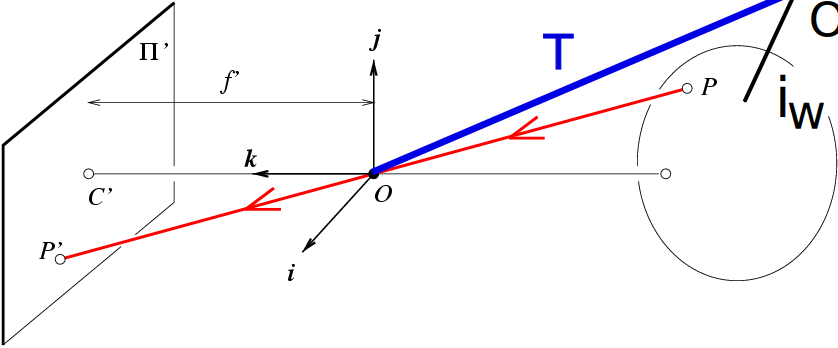
\includegraphics[width=0.9\textwidth]{FIGURES/orientedtranslatedcam1}
%   \end{center}
% \end{frame}

% \begin{frame}
%   \frametitle{Translating Coordinate System}
%   \begin{center}
%    
\includegraphics[width=0.9\textwidth]{FIGURES/translation3D} 
%   \end{center}
%   Assume $O'$ at coordinates $(x_{O'},y_{O'},z_{O'})$ in coordinate system
%   $(O,\bi,\bj,\bk)$ and $P$ has coordinates $(x,y,z)$ also in $(O,\bi,\bj,\bk)$.
%   What are its coordinates in $(O',\bi,\bj,\bk)$?
%  \end{frame}


%  \begin{frame}
%    \begin{itemize}
%    \item Let $(x',y',z')$ its coordinates in $(O,\bi,\bj,\bk)$.
%    \item Write $\overrightarrow{O'P}$ = $\overrightarrow{OP} - \overrightarrow{OO'}$
%    \item Develop:
%      $$
%      \begin{bmatrix}
%        x'\\y'\\z'
%      \end{bmatrix}
%      = 
%      \begin{bmatrix}
%        x\\y\\z
%      \end{bmatrix}
%      -
%      \begin{bmatrix}
%        x_{O'}\\y_{O'}\\z_{O'}
%      \end{bmatrix}
%      =
%      \begin{bmatrix}
%        x-x_{O'}\\y-y_{O'}\\z-z_{O'}
%      \end{bmatrix}
%      $$
%    \item Transformation in homogeneous coordinates:
%      $$
%      \begin{bmatrix}
%        x'\\y'\\z'\\1
%      \end{bmatrix}
%      =
%      \begin{bmatrix}
%        1 & 0 & 0 & -x_{O'}\\
%        0 & 1 & 0 & -y_{O'}\\
%        0 & 0 & 1 & -z_{O'}\\
%        0 & 0 & 0 & 1
%      \end{bmatrix}
%      \begin{bmatrix}
%        x\\y\\z\\1
%      \end{bmatrix}
%      $$
%    \end{itemize}
%  \end{frame}


%  \begin{frame}
%    \frametitle{Rotating Coordinate System}
%    \begin{columns}
%      \column{0.5\textwidth}
%      \begin{center}
%        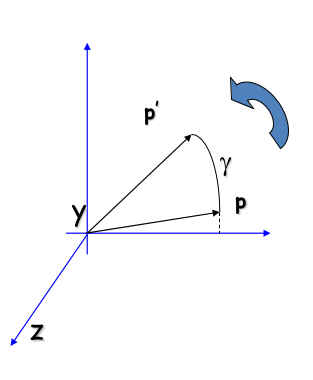
\includegraphics[width=\textwidth]{FIGURES/rotation3d}
%      \end{center}
%      \column{0.5\textwidth}
%      Rotations along coordinate axes
%      $$
%      R_{x\alpha} = 
%      \begin{bmatrix}
%        1 & 0 & 0\\
%        0 & \cos\alpha & -\sin\alpha\\
%        0 & \sin\alpha & \cos\alpha
%      \end{bmatrix}
%      $$
%      $$
%      R_{y\beta} = 
%      \begin{bmatrix}
%        \cos\beta & 0 & -\sin\beta\\
%        0 & 1 & 0\\
%        \sin\beta & 0 & \cos\beta
%      \end{bmatrix}
%      $$
%      $$ 
%      R_{y\gamma} = 
%      \begin{bmatrix}
%        \cos\gamma & -\sin\gamma & 0\\
%        \sin\gamma & \cos\gamma & 0\\
%        0 & 0 & 1
%      \end{bmatrix}
%      $$
%    \end{columns}~\\
%    ~\\
%    Can also be written in homogeneous coordinates
%  \end{frame}
 
%  \begin{frame}
%    \frametitle{Camera Matrix}
%    \begin{itemize}
%    \item Combine world vs camera coordinates with
%    \item Simple Camera matrix and 
%    \item Image plane transformation (axis scalings, shear, translation)
%      $$
%      {\bf C} = {\bf K} \left[{\bf  R}\,\, {\bf t}\right]
%      $$
%    \item ${\bf K}$ $3\times 3$ matrix encoding the homogeneous transformations
%      inside the camera: \myemph{calibration matrix}.
%    \item $\left[{\bf R}\,\, {\bf t}\right]$ Concatenation of world
%      coordinates rotation and origin translation to align camera and
%      world coordinates.
%    \end{itemize}
%    $$
%    w
%    \begin{bmatrix}
%      u\\b\\1
%    \end{bmatrix}
%    = \udesc{{\bf K}}{
%      \begin{bmatrix}
%        \alpha & s & u_0\\
%        0 & \beta & v_0\\
%        0 & 0 & 1
%      \end{bmatrix}}
%    \udesc{\left[{\bf R}\,\, {\bf t}\right]}{
%      \begin{bmatrix}
%        r_{11} & r_{12} & r_{13} & t_x\\
%        r_{21} & r_{22} & r_{23} & t_y\\
%        r_{31} & r_{32} & r_{33} & t_z\\
%      \end{bmatrix}}
%    \begin{bmatrix}
%      x\\y\\z\\1
%    \end{bmatrix}
%    $$
%  \end{frame}
 

%  \begin{frame}
%    \frametitle{Geometric Calibration}
%    \begin{itemize}
%      \item Computing the camera matrix is called geometric calibration.
%      \item Extrinsic parameters: usually easy.
%      \item Calibration focuses more on intrinsic parameters (calibration matrix ${\bf K}$).
%      \item Often difficult.
%    \end{itemize}
%    \begin{columns}
%      \column{0.5\textwidth}
%      \begin{center}
%        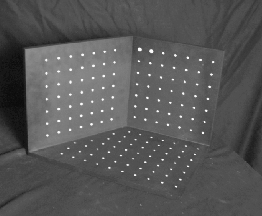
\includegraphics[width=0.8\textwidth]{IMAGES/calibrationobject}
%      \end{center}
%      \column{0.5\textwidth}
%      \begin{itemize}
%      \item Use an object with known geometry
%      \item Use vanishing points / lines
%      \item Use other cues...
%      \end{itemize}
%    \end{columns}
%  \end{frame}


%  \begin{frame}
%    \begin{center}
%      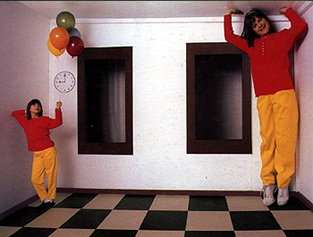
\includegraphics[width=0.8\textwidth]{IMAGES/amesroom}
%    \end{center}
%    Without knowledge of object geometry, calibration can be very problematic (Ames Room illusion).
%  \end{frame}


\section{More on Camera Models}


\begin{frame}
  \frametitle{Shrinking the aperture}
  \begin{center}
    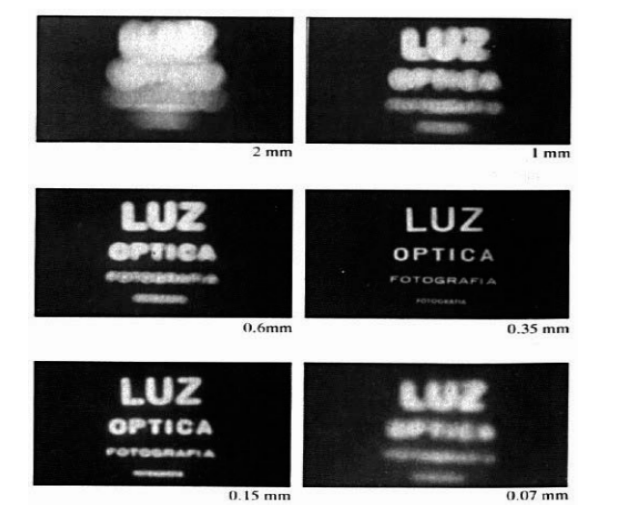
\includegraphics[width=0.7\textwidth]{IMAGES/shrinkingaperture}
  \end{center}
  Less light in, diffraction. 
\end{frame}


\begin{frame}
  \frametitle{Adding Lens}
   \begin{center}
    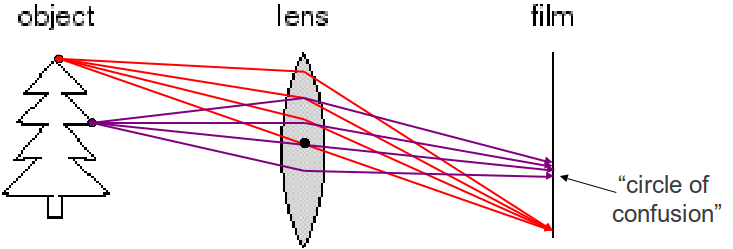
\includegraphics[width=0.7\textwidth]{FIGURES/addinglens}
  \end{center}
  \begin{itemize}
  \item Specific distance for which objects are in focus
  \item Changing shape of lens changes the focus distance.
  \end{itemize}
\end{frame}


\begin{frame}
  \frametitle{Focal Length, Aperture, Depth of Field}
  \begin{center}
    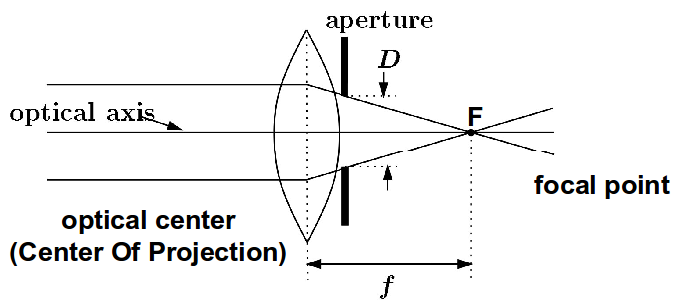
\includegraphics[width=0.9\textwidth]{FIGURES/focallength}
  \end{center}
  \begin{itemize}
  \item Lens focuses parallel rays into a single point.
  \item Aperture restricts range of rays.
  \end{itemize}
\end{frame}


\begin{frame}
  \frametitle{The Eye is a Camera with Lens}
    \begin{center}
    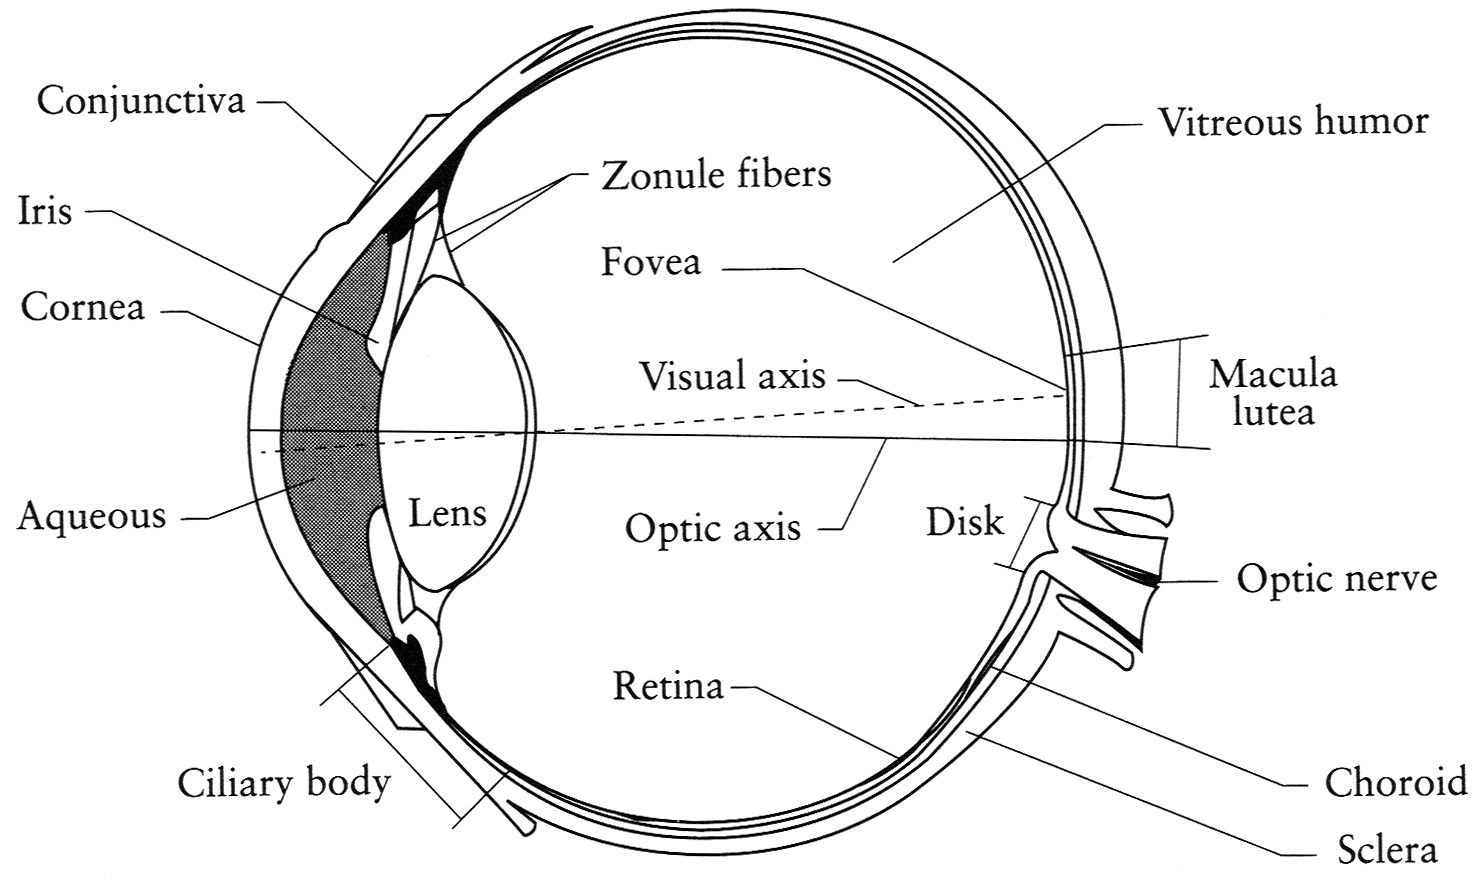
\includegraphics[width=0.9\textwidth]{FIGURES/theeye}
  \end{center}
\end{frame}

\begin{frame}
  \frametitle{Depth of Field}
  \begin{center}
    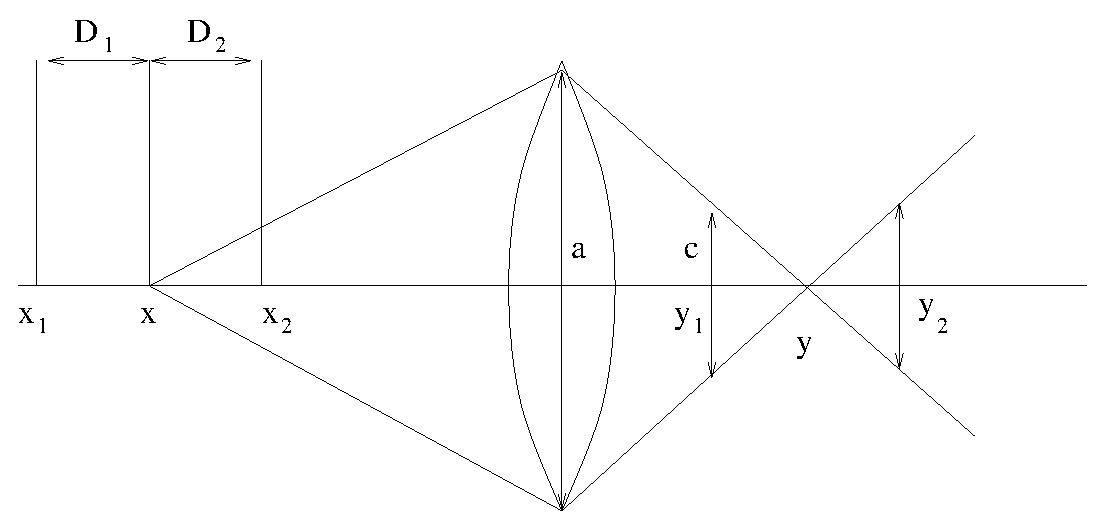
\includegraphics[width=0.9\textwidth]{FIGURES/depthoffield}
  \end{center}
  Controlled by aperture size and focal length.
\end{frame}

% \section{Stereo}




\section{Orthographic Camera}

\begin{frame}[t]{Orthographic Camera}
  \begin{center}
    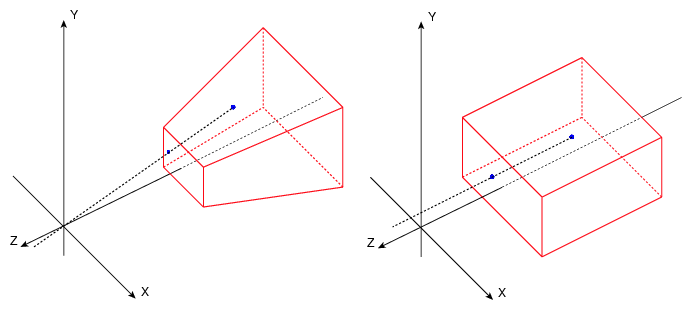
\includegraphics[width=0.9\textwidth]{FIGURES/orthographic}
  \end{center}
  \begin{itemize}
  \item Non physical: ``Camera at infinity'', parallel beams.
  \item Projection Matrix:
    $$
    \Pi =
    \begin{bmatrix}
      1 & 0 & 0\\
      0 & 1 & 0
    \end{bmatrix}
    $$
  \item Useful for ``far objects''. In Some Transmission Imaging too, e.g. CT Scanning, Transmission Electron Microscopy... 
  \end{itemize}
\end{frame}


\begin{frame}[t]{What It Preserves}
  \begin{itemize}
  \item Parallel lines.
  \item Size.
  \item Other?
  \item Matrix in homogeneous coordinates:
    $$
    \Pi =
    \begin{pmatrix}
      1 & 0 & 0 & 0\\
      0 & 1 & 0 & 0\\
      0 & 0 & 0 & 0\\
      0 & 0 & 0 & 1
    \end{pmatrix}
    $$ 
  \item Observe: null determinant!
  \item Utility: Distance preserving drawings, and Wednesday!
  \end{itemize}
\end{frame}





\section{Wednesday}

\begin{frame}[t]{Wednesday}
  \begin{itemize}
  \item Image and Light.
  \item Light / Shading / Reflectance.
  \item Photometric Stereo.
  \end{itemize}
  
\end{frame}


\begin{frame}
   \begin{center}
    
\includegraphics[width=0.75\textwidth]{IMAGES/tiredblock}
  \end{center}
\end{frame}

\end{document}

















% \section{Lighting Models}


% \begin{frame}[t]{Light and Image Formation}
%   \begin{columns}
%     \begin{column}{0.5\textwidth}
%       \begin{center}
%         \fbox{
%           \only<1>{
\includegraphics[width=0.9\textwidth]{FIGURES/imform_obj}}
%           \only<2>{\includegraphics[width=0.9\textwidth]{FIGURES/imform_obj_cam}}
%           \only<3>{\includegraphics[width=0.9\textwidth]{FIGURES/imform_obj_cam_light}}
%           \only<4->{\includegraphics[width=0.9\textwidth]{FIGURES/imform}}
%         }
%       \end{center}
%     \end{column}
%     \begin{column}{0.5\textwidth}
%       \begin{block}{Ingredients}
%         \begin{itemize}[<+->]
%         \item Object
%         \item Camera
%         \item Light source
%         \item Light reflection by object surface.
%         \end{itemize}
%       \end{block}
%     \end{column}
%   \end{columns}
%   ~\vspace{0.5cm}\\
%   \begin{itemize}[<+->]
%   \item Image formation inside camera: when light, scene and camera parameters known: reflectance function.
%   \item BTW: Camera detectors react almost truly linearly to received luminance. \pause
%   \item Can image formation model give enough information about the object surface to reconstruct it?
%   \end{itemize}
% \end{frame}


% \begin{frame}[t]{Bidirectional Reflectance Distribution Function -- BRDF}
%   \begin{center}
%     \includegraphics[width=0.456\textwidth]{FIGURES/reflectance}
%   \end{center}
%   \pause
%   \begin{itemize}
%   \item Luminance emitted by punctual object $\bx$ on a surface $\Ss$
%     with normal direction $\bn(\bx)$ at $\bx$, in emission direction $\bv$
%     characterized by spherical angles $(\theta_e,\phi_e)$ w.r.t $\bn(\bx)$:
%     $$
%     L(\bx,\theta_e,\phi_e)
%     =\int_{\theta_i=0}^{\frac\pi2}\int_{\phi_i=0}^{2\pi}\kappa(\bx,\theta_i,\phi_i,\theta_e,\phi_e)
%     \bar{L}(\theta_i,\phi_i)\sin\theta_i\cos\theta_i\,d\theta_id\phi.
%     $$
%     \pause
%   \item Nice formula but I won't explain what it means!
%   \end{itemize}
% \end{frame}


% \begin{frame}{Specular Vs. Matte Objects} 
%   \begin{center}
%     \includegraphics[width=0.6\textwidth]{FIGURES/specular_diffuse_reflection}
%   \end{center}
%   Two standard reflection models: specular: mirror like surface, diffuse: rough surface (at very small scale): Lambertian model.
%   Others, especially useful in Computer Graphics.
% \end{frame}


% \begin{frame}
% \frametitle{Lambert's Cosine Law}
% \begin{block}{Reflectance}
% \begin{itemize}
%   \item Linearised Lambertian model: $I(\mathbf{p}) = \rho(\mathbf{x}) \mathbf{s}(\mathbf{x}) \cdot \mathbf{n}(\mathbf{x})$
%   \item $\rho({\bf x})$ is the \emph{albedo} at ${\bf x}$ -- material light absorption property, $\rho\in [0,1]$.
%   Assumes matte material such as chalk... 
% \end{itemize}
% \end{block}
% \begin{columns}
%  \begin{column}{0.45\textwidth}
%  \begin{center} 
%  \uncover<2->{\includegraphics[width=0.9\textwidth]{FIGURES/lambertslaw1}}
%  \end{center}
%  \end{column}
%  \begin{column}{0.51\textwidth}
%  \begin{center}
%  \uncover<3->{\includegraphics[width=0.9\textwidth]{FIGURES/lambertslaw2}}
%  \end{center}
%  \end{column}
%  \end{columns}
%  \uncover<4->{ 
%    \begin{block} {In words}
%      \begin{itemize}
%      %\item Only a percentage of received light is reflected, the rest is absorbed by material: albedo.
%      \item Local orientation of object w.r.t. light: In surface 1:
%        surface area matches ray ``section''. In surface 2: surface
%        area larger than ray section, but receive same amount of light.
%      \end{itemize}
%    \end{block}
%  }
% \end{frame}



% \section{Photometric Stereo}



% \begin{frame}
%   \frametitle{The Photometric Stereo (PS) Problem [Woodham, 1980]}
%   \begin{columns}
%     \begin{column}{0.5\textwidth}
%       \begin{center}
%         \fbox{
%           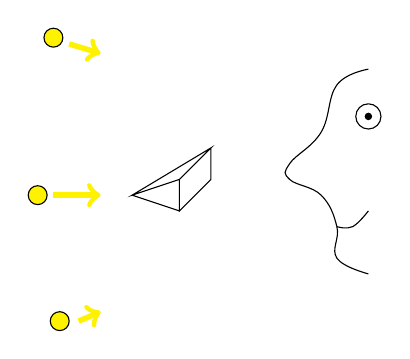
\begin{tikzpicture}[scale=0.4]
% La camera
\path[draw] (-0.5,0)--(1,-0.5)--(1,0.5)--(-0.5,0)--(2,1.5)--(1,0.5)--(1,-0.5)--(2,0.5)--(2,1.5);

% Les trois soleils
\uncover<2->{
\draw[fill=yellow] (-3,5) circle(0.3);
\draw[->,line width=2pt, yellow] (-2.5,4.8)--(-1.5,4.5);
}
\uncover<3->{
\draw[fill=yellow] (-3.5,0) circle(0.3);
\draw[->,line width=2pt, yellow] (-3,0)--(-1.5,0);
}
\uncover<4->{
\draw[fill=yellow] (-2.8,-4) circle(0.3);
\draw[->,line width=2pt, yellow] (-2.2,-4)--(-1.5,-3.7);
}



% Contour d'une tete
\draw  plot[smooth, tension=.7] coordinates {(7,4) (6,3.5) (5.5,2) (4.5,1) (4.5,0.5) (5.5,0) (6,-1) (6,-2) (7,-2.5)};
% Yeux
\draw (7,2.5) circle(0.4);
\draw[fill] (7,2.5) circle(0.1);
% Bouche
\draw  plot[smooth, tension=.7] coordinates {(6,-1) (6.5,-1) (7,-0.5)};

\end{tikzpicture}
%         }
%       \end{center}  
%     \end{column}
%     \begin{column}{0.5\textwidth}
%       \begin{itemize}
%       \item $1$ \myemph{fixed camera} + $1$ ``fixed'' scene
%       \item $m$ lightings
%       \end{itemize}
%       \begin{block}{Goal:}<5>
%         {3D-reconstruction} of the scene from the 2D images
%       \end{block}
%     \end{column}
%   \end{columns}
%   \begin{columns}
%     \begin{column}{0.22\textwidth}
%       \begin{center} 
%         \uncover<2->{\includegraphics[width=0.9\textwidth]{FIGURES/Face01_1}}
%       \end{center}
%     \end{column}
%     \begin{column}{0.22\textwidth}
%       \begin{center}
%         \uncover<3->{\includegraphics[width=0.9\textwidth]{FIGURES/Face01_2}}
%       \end{center}
%     \end{column}
%     \begin{column}{0.22\textwidth}
%       \begin{center}
%         \uncover<4->{\includegraphics[width=0.9\textwidth]{FIGURES/Face01_3}}
%       \end{center}
%     \end{column} 
%     \begin{column}{0.22\textwidth}
%       \begin{center}
%         \uncover<5->{\includegraphics[width=0.9\textwidth]{FIGURES/Face01_shape}}
%       \end{center}
%     \end{column}  
%   \end{columns} 
%   {\fontsize{5}{5}\selectfont Slide by Y. Qu{\'e}au}
% \end{frame}


% \begin{frame}[t]{Settings}
%   \begin{itemize}
%   \item Representation of the surface. Assume surface parameterized by $(u,v)\mapsto \Ss(u,v)\in \RR^3$. Even better: \myemph{depth map}:
%     $$
%     S(u,v) = [u,v,z(u,v)]^T:\text{ Monge Patch}.
%     $$
%   \end{itemize}
%   \pause
%   \begin{columns}
%     \begin{column}{0.38\textwidth}
%       \begin{center}
%         \uncover<2->{\includegraphics[width=1.0\textwidth]{FIGURES/surfacediffgeom}}
%       \end{center}      
%     \end{column}
%     \begin{column}{0.62\textwidth}
%       Tangent vectors at $\bx(u,v) = [u,v,z(u,v)]^\top$
%       $$
%       \pder{\Ss}{u}=S_u=
%       \begin{bmatrix}
%         1\\ 0\\ \pder{z}{u}
%       \end{bmatrix},\quad
%       \pder{\Ss}{v}=\Ss_v
%       \begin{bmatrix}
%         1\\ 0\\\pder{z}{v}
%       \end{bmatrix},\quad
%       $$      
%     \end{column}
%   \end{columns}
% \pause
%   \begin{itemize}
%   \item Normal vector $\bn(u,v) = \bn(\bx(u,v))$
%     $$
%     \bn(\bx) = \frac{\Ss_u\times\Ss_v}{|\Ss_u\times\Ss_v|} = \frac{1}{\sqrt{|\nabla z|^2 + 1}}
%       \begin{bmatrix}
%         z_u\\z_v\\-1
%       \end{bmatrix}
%     $$
%   \end{itemize}
% \end{frame}


% \begin{frame}[t]{Shape From Shading (SFS) B. Horn 1970}
%   \begin{itemize}
%   \item Problem: Observed image I from a camera.
%   \item Can I infer shape of imaged object from Image Value?
%   \item Very complicated problem, \myemph{ill-posed}. 
%   \item A problem is called \myemph{Well-Posed} in the sense of
%     Hadamard if, for a given datum, it has a unique solution and if
%     the solution depends continuously on the datum.
%   \item A problem is called \myemph{Ill-Posed} if it is not well-posed.
%   \item Why is SFS ill-posed?  First: To specify a surface point in 3-space: 3 coordinates and a relation between them: 2 Degrees of freedom, i.e., two unknown.
%   \item 1 observed gray-scale value per point: one equation.
%   \item But I need at least the same number of equations as the number of unknown!
%   \item  And if albedo is not constant / known, I have an extra degree of freedom! 
%   \end{itemize}
% \end{frame}




% \begin{frame}[t]{Woodham Original PS}
%   \begin{itemize}[<+->]
%   \item $m$ far away lights -- parallel beam , known direction and light intensity.\vfill
%   \item Orthographic camera: pixel at position $[u,v]^T$ on image plane:
%     projection of point $[x,y,z] = [u,v,z(u,v)]^T$ on surface $\Ss$ to reconstruct.  \vfill
%   \item Image is matte: Lambert's cosine law describes image formation model. $m$ images $I_1,\dots I_m$ 
%     of surface $ Ss$ with light vector $\bs_i$:
%     $$
%     I_i(u,v) = \rho(u,v)\,\bs_i\cdot\bn(u,v).
%     $$\vfill
%   \item $\bn$ normal vector at $\Ss$ at point $(u,v,z(u,v))$.\vfill
%   \item Can we recover vectors $\bn$, depth map $z(u,v)$, albedo $\rho(u,v)$?\vfill
%   \item Woodham, 1980: Yes under some conditions:
%     \begin{itemize}
%     \item $\rho\not=0$, 
%     \item at least 3 light vectors are not coplanar!
%     \item No shadow. 
%     \end{itemize}

%   \end{itemize}
% \end{frame}





% \begin{frame}
%   \frametitle{Multiple View Correspondences}
%   \begin{center}
%     \includegraphics[width=0.9\textwidth]{FIGURES/stereo}
%   \end{center}
%   If we can recover $x'$ from $x$ we can recover depth.
% \end{frame}

% \begin{frame}
%   \frametitle{Image Correspondence}
%   \begin{center}
%     \includegraphics[width=0.9\textwidth]{IMAGES/stereo2images}
%   \end{center}
%   How do we match points from image 1 to image 2: you should have seen some of it with Kim,
%   but this is not the end of the story!
% \end{frame}


% \begin{frame}
%   \frametitle{Epipolar Constraints}
%   \begin{center}
%     \includegraphics[width=0.9\textwidth]{FIGURES/epipolarconstraint}
%   \end{center}
%   \begin{itemize}
%   \item    Potential match for $x$ must lie in corresponding line $l'$
%   \item  Potential match for $x'$ must lie in corresponding line $l$
%   \end{itemize}  
% \end{frame}


% \begin{frame}
%   \frametitle{Epipolar Constraints}
%   \begin{center}
%     \includegraphics[width=0.9\textwidth]{FIGURES/epigeom}
%   \end{center}
%   \begin{itemize}
%   \item  Line connecting $O$ and $O'$: \myemph{baseline}
%   \item Plane through baseline $x$ and $x'$: \myemph{Epipolar Plane}
%   \item Epipoles: intersection of baseline and image planes:
%     projection of the other camera center.
%   \item Epipolar Lines - intersections of epipolar plane with image
%     planes (always come in corresponding pairs)
%   \end{itemize}  
% \end{frame}


% \begin{frame}
%   \frametitle{Example: Converging cameras}
%   \begin{center}
%      \includegraphics[width=0.9\textwidth]{FIGURES/convergecam}
%   \end{center}
% \end{frame}

% \begin{frame}
%   \frametitle{Calibrated Case}
%    \begin{center}
%     \includegraphics[width=0.65\textwidth]{FIGURES/epicalibrated}
%   \end{center}
%   Camera parameters known for the two cameras: calibration matrices $K$ and $K'$\\
% \end{frame}

% \begin{frame}
%   \begin{itemize}
%   \item  $x$ and $x'$ (in 3D coords but not the same)  are related by rotation and translation.
%     $$x' = R(x-\bt)$$
%   \item Their homogeneous coordinates $y$ and $y'$ are related by a simple matrix $E$ built from $R$ and $t$
%     $$
%     y^T E y = 0.
%     $$
%   \item $E$ is called the \myemph{essential matrix} (Longuet-Higgins 1981).
%   \item $E$ can be estimated from images.
%   \item The position and orientation of camera 1 vs camera 2 (i.e.,
%     $R$ and $\bt$) can be recovered from $E$.
%   \end{itemize}
% \end{frame}

% \begin{frame}
%   \frametitle{Note on the geometric transformation between image 1 and
%     image2}
%   \begin{itemize}
%   \item The transformation between $y$ and $y'$ is not linear: it is
%     an \myemph{homography} between the 2 image planes: 
%   \item An homography conserves straight lines, but not parallelism. 
%   \item Two parallel lines intersect at infinity: after an homography they may intersect at finite distance.
%   \end{itemize}
% \end{frame}


% \begin{frame}
%    \frametitle{Uncalibrated Case}
%    \begin{itemize}
%    \item No way to directly compare $x$ and $x'$: they relate through
%      the unknown transformations $K$ and $K'$.
%    \item A relation however still exists (Faugeras, Luong, 1992)
%      $$
%      y^T \udesc{F}{K^{-\top} E K'^{-1}} y =0
%      $$
%    \item $F$ is called the \myemph{fundamental matrix}. 
%    \item Though $K$ and $K'$ are unknown $F$ can be \myemph{esitimated}
%      (complicated) thus used for the correspondence problem!
%    \item {\small $K^\top$ is the transposed of $K$: inverse row and line indices.
%      For a vector in column, write it in line.}
%    \item {\small $K^{-1}$ is the inverse of $K$: provides the inverse change
%      of coordinates from unnormalized to normalized image coordinate.}
%    \item {\small $K^{-\top}$ means inverse of the transposed matrix: The same
%      as transposed of the inverse.}
%    \end{itemize}
% \end{frame}
